\documentclass[11pt]{article}
% Sets page layout with 0.5-inch margins and letter paper size
\usepackage[letterpaper, tmargin=0.75in,bmargin=1in,rmargin=0.5in,lmargin=0.5in]{geometry}
% Ensures proper font encoding for output, improving character representation and hyphenation
\usepackage[T1]{fontenc}
\usepackage{float}
% Loads Latin Modern fonts for high-quality typography
\usepackage{lmodern}
% Enhances text appearance with micro-typographic improvements like kerning and spacing
\usepackage{microtype}
% Provides advanced mathematical typesetting tools and additional math symbols
\usepackage{amsmath, amssymb}
% Enables inclusion and manipulation of external graphics
\usepackage{graphicx}
% Nice tables
\usepackage{makecell}
\usepackage{booktabs}
% Customizes page headers and footers
\usepackage{fancyhdr}
% Allows formatting of section titles
\usepackage{titlesec}
% Provides control over line spacing (e.g., single, one-and-a-half, double)
\usepackage{setspace}
% natbib setup for author-year citation style 
\usepackage[authoryear]{natbib}
\bibpunct{(}{)}{;}{a}{,}{,}
% Enables clickable hyperlinks for references within the document.
\usepackage{hyperref} 
% Allow long URLs (e.g., in footnotes) to break across lines cleanly
\usepackage{xurl}
% Allows control of section heading styling
\usepackage{sectsty}
\pagestyle{fancy}
% Increase headheight to accommodate logo
\setlength{\headheight}{0.3in}
%for block diagram at the beginning of methodology
\usepackage{tikz}
\usetikzlibrary{shapes.geometric, arrows, positioning}
%for my tables
\usepackage{multirow}
\usepackage[normalem]{ulem}

\pagestyle{fancy}
\raggedbottom


\setlength{\intextsep}{0pt}
\usepackage{abstract}
\renewcommand{\abstractname}{}    % Clear the title text
\renewcommand{\absnamepos}{empty} % Remove the space where the title was

%Add page number in the footer (e.g., centered)
\renewcommand{\footrulewidth}{0.2pt}
\renewcommand{\headrulewidth}{0.2pt}
\rfoot{\footnotesize{\thepage}}
\cfoot{}
\usepackage{booktabs}
\usepackage{tabularx}
\usepackage{amsmath}
\usepackage{xcolor}
\usepackage{hyperref}
\usepackage{pgfplots}
\usepgfplotslibrary{statistics}
\pgfplotsset{compat=1.16}
\usepackage{subcaption}
\rhead{\footnotesize{\textit{October, 2026}}}
\lhead{\footnotesize{\textit{26F-ECON-430, Project 1}}}
\begin{document}

\begin{center}
\Large{Report on S\&P 500 Stock Market Volatility During the Great Recession.}

\vspace{0.2in}

\large{Olivia Gallagher, Yamini Sirobushanam, Zoe Scherrer}
\end{center}
\section{Economic Theory and Hypothesis}
\subsection{Introduction}
\indent The Great Recession of 2008 is among the most notable economic downturns in recent history. Although disproportionate, recessions negatively impact \textit{everyone}, rich or poor, through income loss, unemployment, and financial uncertainty. During the second quarter of 2025, stock holdings accounted for 45\% of American households’ financial assets.\footnote{\cite{CNN}} Therefore, understanding how recessions impact financial markets is crucial to protecting the financial security of Americans. In this report, we will investigate how S\&P 500 stock market volatility changed during the Great Recession (2008) by comparing the volatility from the years prior to the recession (2000-2008), to the years following (2008-2014).
\subsection{Relevant Economic Theory}
\indent The price of a given stock is determined by the respective company's expected future earnings, growth, and perceived risk. During recessions, consumer spending naturally drops due to a decreased amount of personal funds. Reduced consumer spending lowers sales revenue, resulting in decreased corporate profits. This can instill skepticism in investors of future corporate earnings, affecting stock valuation. Stocks prices can jump or drop in short periods of time, increasing volatility.\footnote{\cite{Fidelity}} Uncertainty of stock performance limits companies' ability to raise capital through issuing stocks and bonds. As a result, corporations issue layoffs and unemployment rises. \\
\indent G. William Schwert from the National Bureau of Economic Research (NBER) discovered that during the Great Depression, the monthly standard deviation of stock prices were 50\% larger in 1929 than usual.\footnote{\cite{NBER}} Standard deviations are a useful measure to quantify how different stock prices are from their typical average. Schwert also notes that the increase in volatility did not disappear quickly, but rather persisted for a longer period of time than expected. While the recession was not the sole cause of the volatility, the findings underscore how economic uncertainty can correlate with financial market fluctuations. \\
\indent The same pattern Schwert discovered is still prevalent in economic downturns today. A researcher at San Diego State University (SDSU) evaluated financial markets during the Covid-19 pandemic in 2020, and confirms that the massive unpredictability leads to huge drops in corporate revenues and stock valuations.\footnote{\cite{sdsu2020volatile}} During the pandemic, corporate profits drastically decreased worldwide. The economy underwent significant changes, creating widespread uncertainty of future projections. As a result, stock prices substantially changed (increased \textit{and} decreased) to reflect lower consumer spending and corporate earnings. By studying the 2008 Great Recession, we aim to explore how stock market volatility evolved during a major macroeconomic downturn, building on existing research to further understand the relationship between economic instability and financial market behavior.
\subsection{Hypothesis and Expected Effects}
We hypothesize that the Great Recession was associated with increased stock market volatility. Therefore, our null hypothesis is that the recession had no statistically significant effect on S\&P 500 volatility, while our alternative hypothesis is that the recession increased volatility. To formulate our statistical models, we consider five predictors: the Consumer Price Index (CPI), Gross Domestic Product (GDP) which we calculate as GDP growth,  the change in unemployment rate (Un. Rate Change) and the Federal Reserve interest rate (Fed. Reserve IR Change), which are both calculated as difference in absolute change, and the Consumer Confidence Index (CCI). To explain how these predictors work together to estimate volatility, we begin by examining their expected effects on corporate profits. \\
\indent \textbf{CPI} is used as a key economic indicator to measure inflation. Unexpected inflation can create uncertainty about interest rates. If \textbf{the Fed. Reserve IR Change} increases, borrowing costs for businesses and consumers could increase. Businesses could face higher costs for materials, product transportation, and even wages. To combat increased operation costs, businesses must increase their prices to keep their profit. If they fail to do so, their profit shrinks. Additionally, higher prices have the potential to lower company sales, negatively impacting profit. \\
\indent When the \textbf{Un. Rate Change} increases, consumers have less money to spend. With a lower demand for goods and services, GDP is expected to decrease. A decrease in \textbf{GDP Growth} reflects a decline in overall economic activity, as fewer goods and services are being produced and sold. Naturally, both translate to a decrease in corporate profits, on average.  \\
\indent The \textbf{CCI} measures how people feel about the economy and their personal financial situations. The index is a good predictor of consumer spending and saving habits. When the index increases, consumers have a positive outlook on the economy, inflation, and their finances, likely increasing consumption. On the contrary, when confidence falls, consumers may reduce their spending which can negatively impact business’ sales and expected profits. \\
\indent All five predictors have the ability to impact corporate earnings. Lower profit margins likely increases investor uncertainty by raising concerns about the company’s ability to generate future profits. If investors are uncertain about how long the economic downturn will last or its impact on businesses, we can expect stock volatility to fluctuate. 
\vspace{0.8em}
\begin{table}[htbp]
\centering
\small
\renewcommand{\arraystretch}{1.35}
\caption{\textbf{Expected Coefficient Signs and Magnitude on S\&P 500 Stock Market Volatility.}}
\label{tab:coefficient_hypotheses}
\vspace{0.8em}
\begin{tabularx}{\textwidth}{l c l X}
\toprule
\textbf{Variable} & \textbf{Sign} & \textbf{Magnitude} & \textbf{Theoretical Rationale} \\
\midrule
Un. Rate Change & $+$ & Large & Rising unemployment curbs consumer spending and corporate earnings, driving up market price volatility. \\
GDP Growth & $-$ & Moderate & Economic growth promotes market stability and earnings predictability, dampening overall volatility. \\
CPI  & $+/-$ & Ambiguous & Unexpected inflation generates policy and purchasing power uncertainty, whereas anticipated shifts have little impacts. \\
Fed. Reserve I.R. Change & $+$ & Moderate & Higher borrowing costs can make companies less likely to invest and lower expectations for future profits, although expected changes in interest rates may lessen this effect.\\
CCI & $-$ & Large & Greater consumer optimism stabilizes future market expectations, reducing sharp fluctuations in stock prices. \\
\bottomrule
    \end{tabularx}
\end{table}
\section{Data Description and Exploratory Analysis}
\subsection{Dataset Description}
The data used in this study are sourced from Kaggle.\footnote{CPI: \cite{KondoroCPI}, GDP:\cite{KondoroGDP}, Unemployment Rate:\cite{KondoroUnemployment}} We have cleaned the years to only contain 2000-2014. Kaggle data are sourced various ways: user uploads, crowdsourcing, corporate sponsors, and partnerships, for example. All Kaggle data has been checked and verified against government data sources. Sourcing data from one place eases pre-processing and creates consistent formatting. \\
\indent \textbf{CPI} measures the change in the average price paid by consumers on goods and services. It can track the cost of these goods over time. Inflation rate is measured by how much CPI has increased or decreased compared to the previous month. Since CPI is an index, we measure the units in points. \textbf{GDP Growth} is a measure of the change in total value of goods and services produced in the United States economy, calculated quarterly, measured in billions of dollars. For this analysis, quarterly GDP was transformed into a growth rate by calculating the percentage change between periods and multiplying the result by 100. This allows GDP to be measured as a percentage growth rate rather than in dollar values. The \textbf{Un. Rate Change} measures the percentage of people in the labor force who are unemployed, and tracks whether it increases or decreases. It is reported monthly and helps indicate the conditions of the labor market. Un. Rate Change is interpreted as percent points. The \textbf{Fed. Reserve IR Change} measures the change in average interest rate that U.S. banks charge one another for overnight loans of excess reserves. The "change" calculates how much the effective federal funds rate increased or decreased compared to the previous month, expressed as a percentage points. As previously stated, \textbf{CCI} is a measure representing consumers’ anticipated future financial situations, predicting their willingness to consume more of their income instead of saving. Values above 100 suggest higher confidence and increased future consumption, while values below 100 indicate lower confidence and more propensity to save. \textbf{S\&P 500 Volatility} represents the amount that S\&P 500 valuation has changed, calculated month-to-month. It is constructed by using the standard deviation of S\&P 500 adjuncted close returns in daily percentages. 
\subsection{Descriptive Statistics and Visualizations}
\begin{table}[H]
\centering
\caption{\textbf{Descriptive Statistics}}
\label{tab:descriptive}
\small
\setlength{\tabcolsep}{4pt}
\begin{tabularx}{\textwidth}{Xrrrrrrrrrr}
\toprule
Variable & Count & Mean & Std & Min & 25\% & 50\% & 75\% & Max & Skew & Kurt. \\
\midrule
CPI & 177 & 205.81 & 20.54 & 170.90 & 185.50 & 207.67 & 224.09 & 237.50 & -- & -- \\
Un. Rate Change & 177 & 0.01 & 0.17 & -0.50 & -0.10 & 0.00 & 0.10 & 0.50 & -- & -- \\
GDP Growth & 177 & 1.00 & 0.75 & -1.95 & 0.62 & 1.13 & 1.40 & 2.45 & -- & -- \\
Fed. Reserve IR Change & 177 & -0.03 & 0.18 & -0.96 & -0.02 & 0.00 & 0.02 & 0.26 & -- & -- \\
CCI & 177 & 99.43 & 1.51 & 96.36 & 98.33 & 99.55 & 100.53 & 102.90 & -- & -- \\
Volatility & 177 & 1.09 & 0.69 & 0.26 & 0.64 & 0.95 & 1.24 & 5.09 & 2.58 & 9.37 \\
\bottomrule
\end{tabularx}
\end{table}
\vspace{0.8em}
In Table 2 above, volatility averages 1.09 with a median of 0.95. The skewness (2.58) and kurtosis (9.37) indicate a strongly right-skewed distribution with heavy tails, meaning most months are calm but a few have extreme jumps. \\
\begin{figure}[H]
    \centering
    \label{fig:placeholder}
    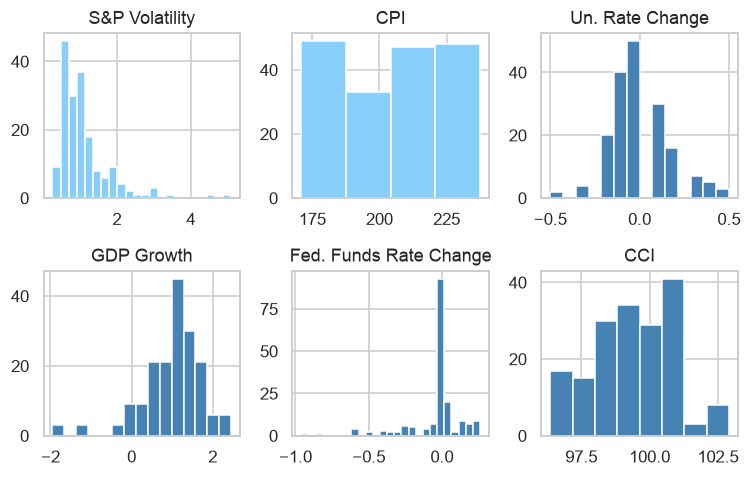
\includegraphics[width=0.75\linewidth]{Histograms.png}
    \caption{\textbf{Histograms}}
\end{figure}
In Figure 1, we use Freedman and Diaconis Histograms to properly display our data with bin  width calculated using the interquartile range of each predictor. 

\begin{figure}[H]
\centering
\begin{tikzpicture}
\begin{axis}[
    width=0.8\textwidth,
    height=8cm,
    ymin=0, ymax=1,
    xmin=0.4, xmax=3.6,
    ymajorgrids=true,
    grid style={gray!30},
    ylabel={Volatility},
    xlabel={Period},
    title={S\&P 500 Volatility by Recession Period},
    xtick={1,2,3},
    xticklabels={Pre-Recession, Great Recession, Post-Recession},
    boxplot/draw direction=y,
    boxplot/box extend=0.8,
]

% Pre-Recession
\addplot+[
    boxplot prepared={
        draw position=1,
        lower whisker=0.035, lower quartile=0.075, median=0.138,
        upper quartile=0.193, upper whisker=0.347
    },
    fill=blue!60!black!70, draw=black!70, mark=o, mark options={fill=white}
] table[row sep=\\, y index=0] {
    0.38 \\ 0.385 \\ 0.40 \\ 0.413 \\ 0.50 \\
};

% Great Recession
\addplot+[
    boxplot prepared={
        draw position=2,
        lower whisker=0.135, lower quartile=0.212, median=0.32,
        upper quartile=0.522, upper whisker=0.872
    },
    fill=blue!60!black!70, draw=black!70, mark=o, mark options={fill=white}
] table[row sep=\\, y index=0] {
    1.0 \\
};

% Post-Recession
\addplot+[
    boxplot prepared={
        draw position=3,
        lower whisker=0.0, lower quartile=0.077, median=0.11,
        upper quartile=0.16, upper whisker=0.28
    },
    fill=blue!60!black!70, draw=black!70, mark=o, mark options={fill=white}
] table[row sep=\\, y index=0] {
    0.325 \\ 0.33 \\ 0.35 \\ 0.365 \\ 0.555 \\
};

% Dashed reference line
\addplot[red!70!black, dashed, thick, no marks] coordinates {(0.4,0.17) (3.6,0.17)};

\end{axis}
\end{tikzpicture}
\caption{\textbf{S\&P 500 Volatility by Recession Period.}}
\label{fig:vol_by_period}
\end{figure}
\vspace{0.8em}
In Figure 2 above, the dashed line marks a mean volatility of 0.17 from min-max scaling. This means that we scale our volatility between 0 and 1, so our mean appears much smaller by default, compared to the total sample volatility mean of 1.09 (Table 2). See box plots for remaining variables in Appendix 7.1. \\
\indent Figure 3 displays a correlation heat map of our predictors. The absolute value of all predictors are below 0.80, so there is no obvious multicollinearity. However, we will confirm the absence of multicollinearity by performing a Variance Inflation Factor (VIF) test, later. Figure 4 displays a scatter plot of key relationships. 
\vspace{0.8em}
\begin{figure}
    \centering
    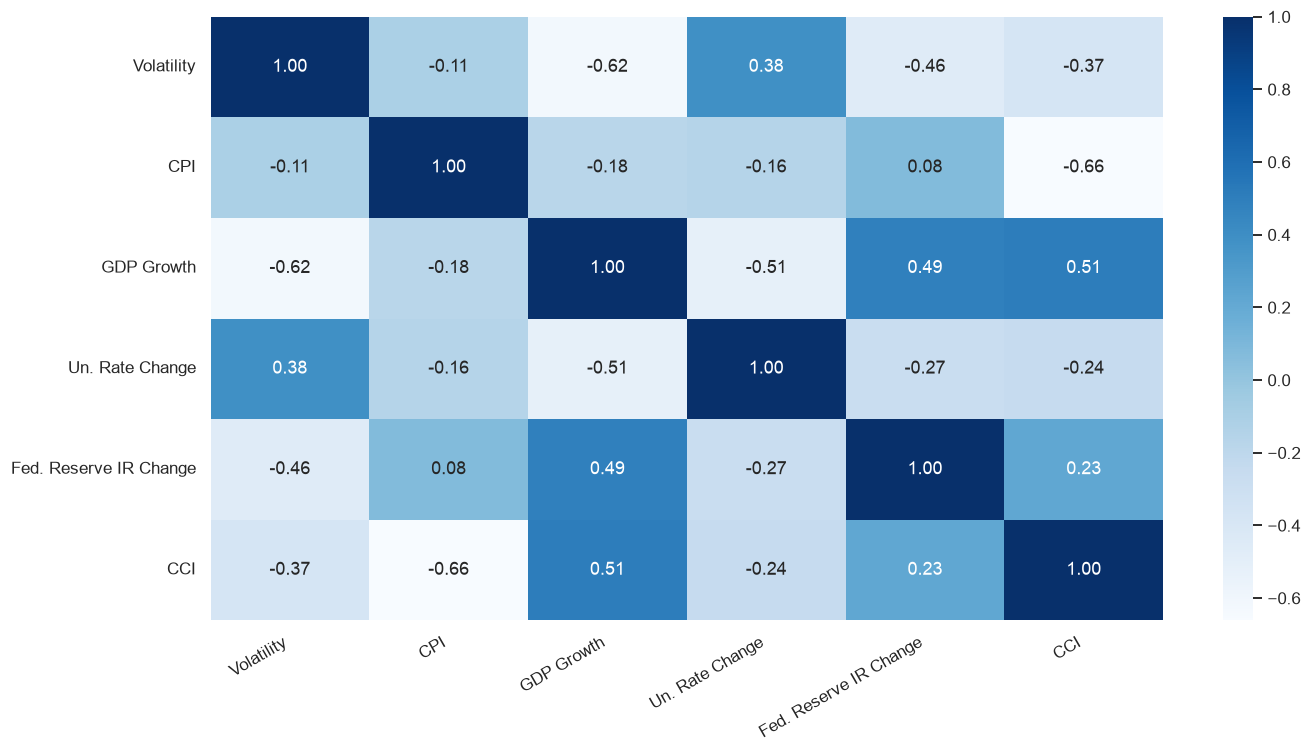
\includegraphics[width=.75\linewidth]{correlation matrix.png}
    \caption{\textbf{Correlation Matrix}}
    \label{fig:placeholder}
\end{figure}

\begin{figure}[H]
    \centering
    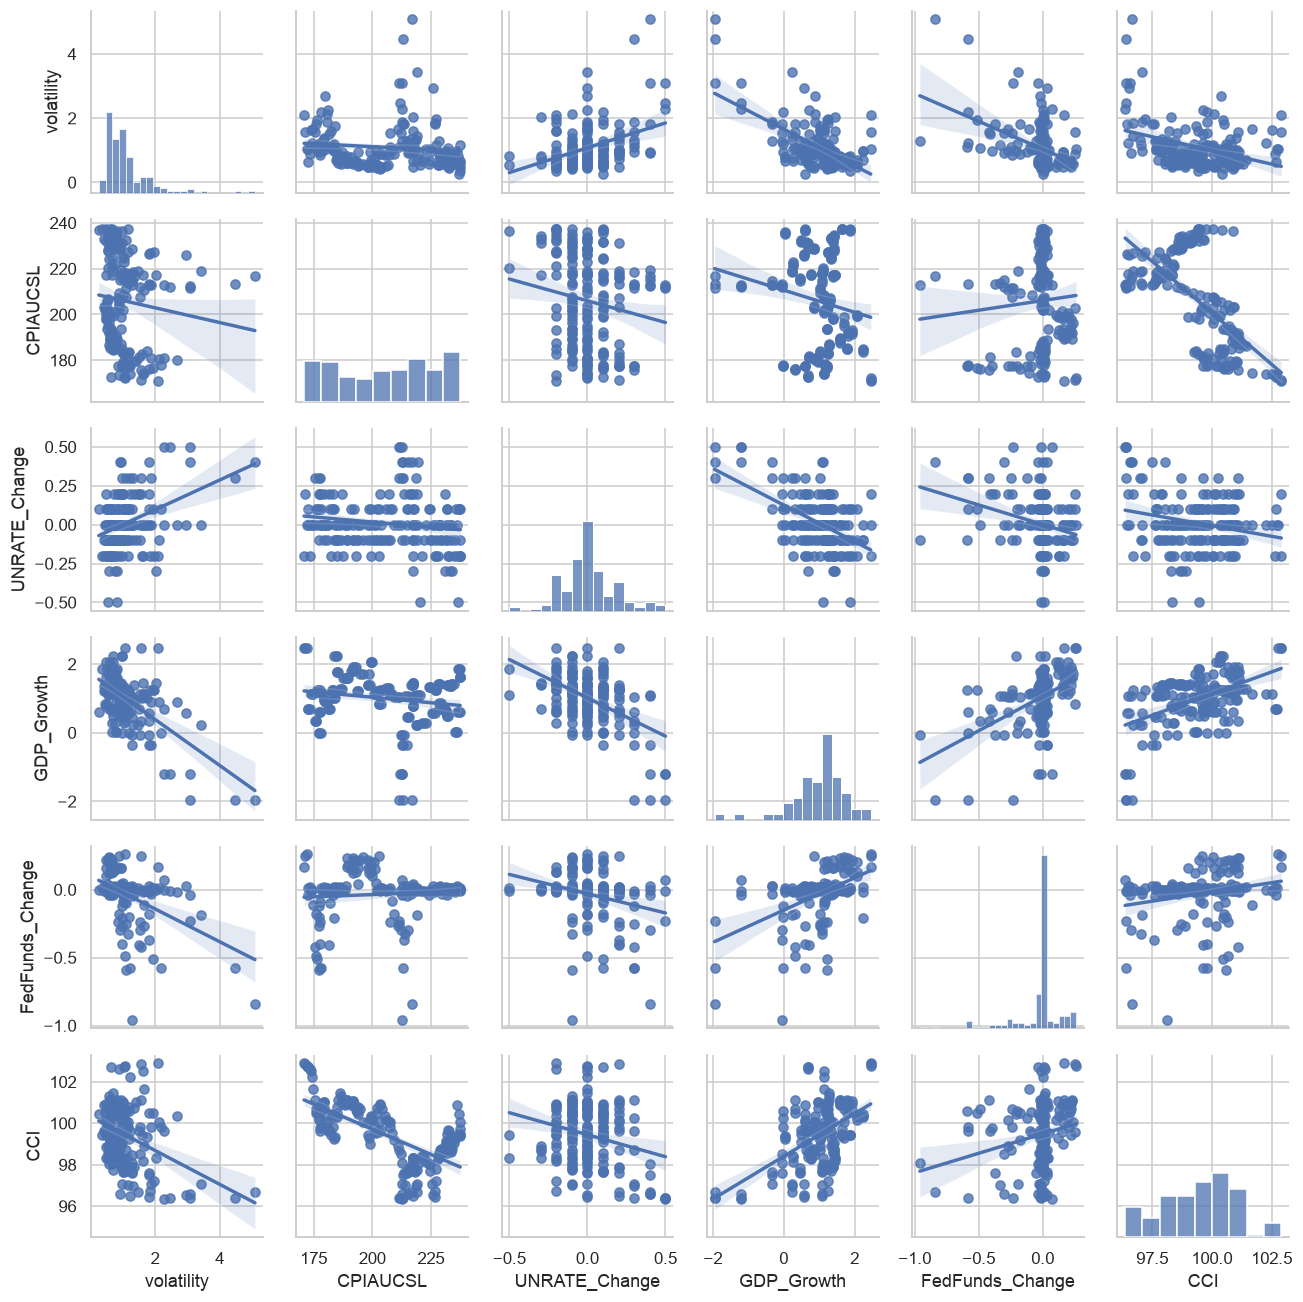
\includegraphics[width=0.60\linewidth]{scatterplot relationships.png}
    \caption{\textbf{Scatter Plot of Key Relationships}}
    \label{fig:placeholder}
\end{figure}


\subsection{Diagnostics and Pre-processing}
\vspace{0.8em}
\begin{figure}[H]
    \centering
    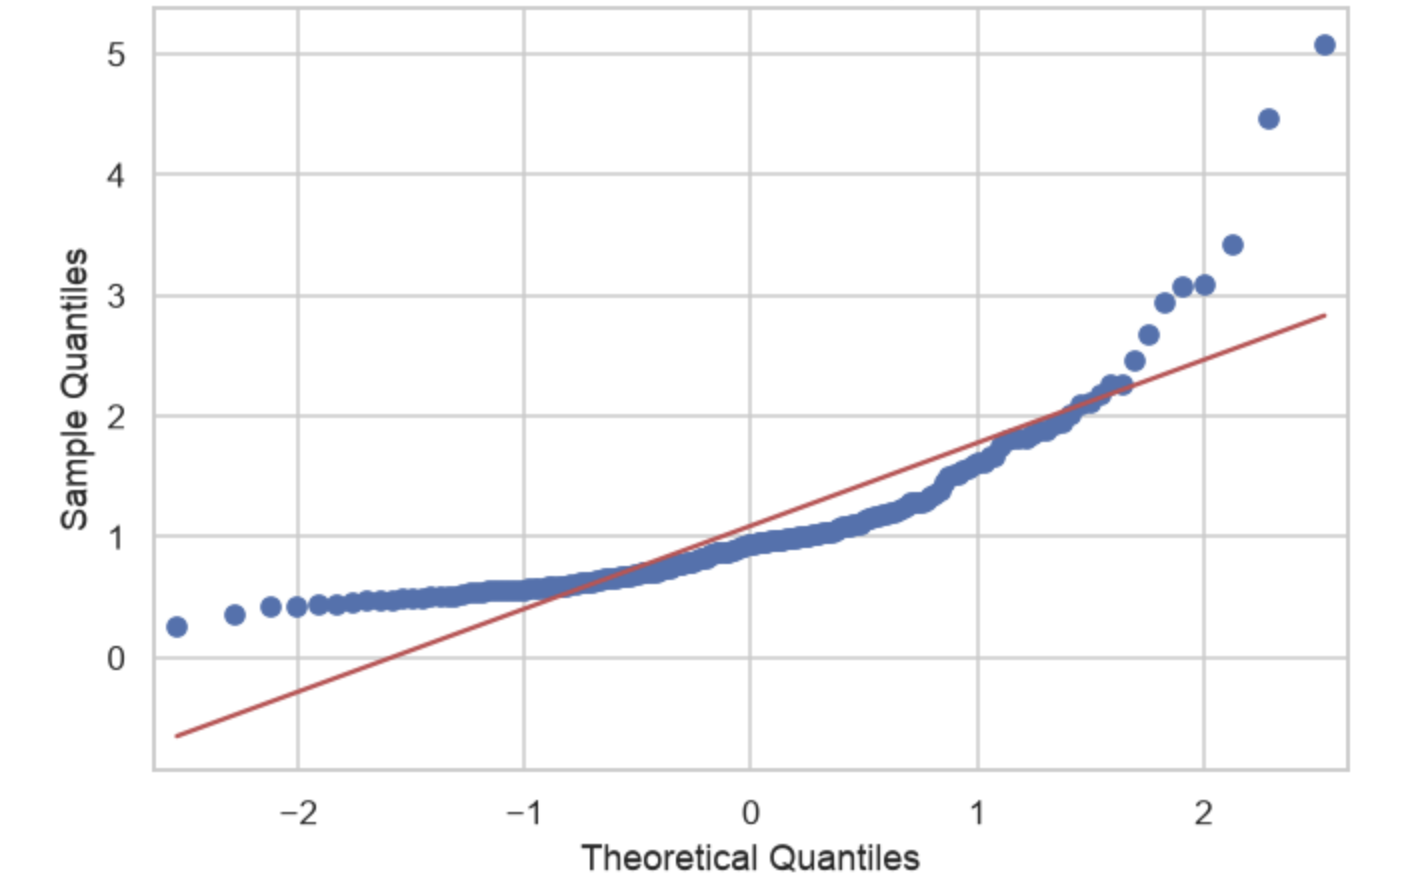
\includegraphics[width=0.5\linewidth]{QQ volatility.png}
    \caption{\textbf{Q-Q Plot: Volatility}}
    \label{fig:placeholder}
\end{figure}
Our dependent variable follows a normal distribution on average. The ends of the plot in Figure 5 show some residuals deviating from the normal distribution. This is reflected in the high skewness of the data (Table 2, 2.58). To see Q-Q and density plots for remaining continuous variables, see Appendix 7.2 and 7.3, respectively. \\
\begin{figure}[H]
    \centering
    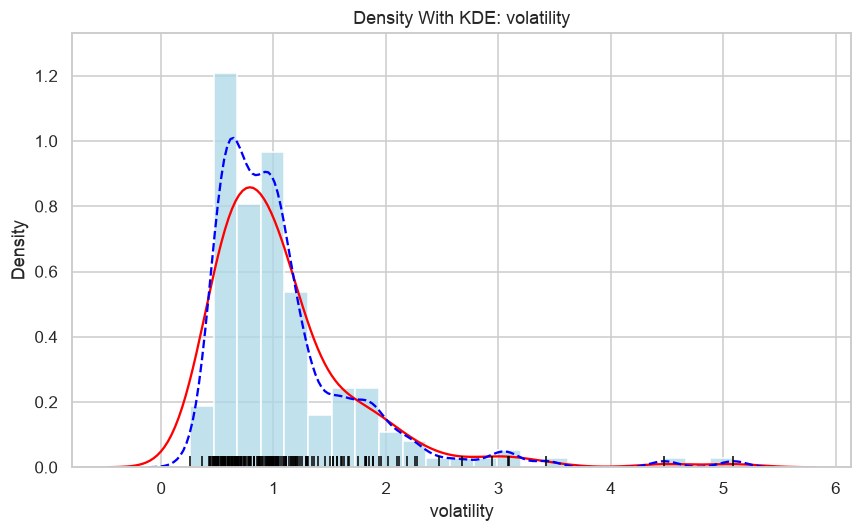
\includegraphics[width=0.75\linewidth]{Volatility Density.png}
    \caption{\textbf{Volatility Density}}
    \label{fig:placeholder}
\end{figure}

\subsection{Exploratory Analysis Discussion}
\indent 
Several transformations were applied to the variables to improve the model specification and account for potential nonlinear relationships. First, GDP was transformed into GDP growth by calculating the monthly growth rate. Since GDP was originally measured quarterly, it was also reindexed to match the frequency of the other predictive variables. This transformation helped address near-perfect multicollinearity between the original GDP variable and CPI, reducing their correlation to -0.18 (Figure 3). Next, the unemployment rate was transformed into monthly changes, Un. Rate Change, using the `.diff()` function. Rather than measuring the level of unemployment, this variable captures the difference between the current and previous month's unemployment rates, expressed in percentage points. This transformation was applied because the original unemployment rate variable was not statistically significant, while the transformed variable is statistically significant in the regression analysis. Similarly, the Effective Federal Funds Rate was transformed into monthly changes (Fed. Reserve IR Change) using the same Python function. The original interest rate variable was not statistically significant, whereas the transformed variable is. Lastly, the S\&P 500 adjusted close price was transformed into daily percentage returns, which were then used to calculate monthly standard deviations and construct our response variable, volatility. This transformation was necessary because our research question focuses on fluctuations in stock market returns rather than changes in the overall value of the S\&P 500. We also considered potential nonlinear relationships, particularly between GDP growth and stock market volatility. The relationship between GDP growth and volatility may vary depending on whether the economy is experiencing periods of expansion or economic hardship. To account for this possibility, we introduced a quadratic term for GDP growth to examine whether a nonlinear specification would better explain the relationship between GDP growth and volatility. \\
\indent To identify potential outliers, the IQR method was applied to monthly S\&P 500 volatility, identifying a total of 11 outliers (Table 3). Seven of these observations occurred between September 2008 and March 2009, during the Great Recession. October 2008 recorded the highest volatility at approximately 5.09, followed by November 2008 at 4.48. Additional outliers were identified in other years, such as 2001 and 2002, which may reflect other periods of economic uncertainty. These observations were not removed because we wanted to preserve the actual fluctuations in stock market returns. Removing these observations could exclude important information about how volatility behaves during periods of financial instability. \\
\begin{table}[H]
\centering
\caption{\textbf{IQR Outliers}}
\label{tab:outliers}
\renewcommand{\arraystretch}{1.3}
\setlength{\tabcolsep}{16pt}
\begin{tabular}{rcc}
\toprule
Obs. & Date & Volatility \\
\midrule
17 & September 2001 & 2.1914 \\
27 & July 2002 & 2.6813 \\
30 & October 2002 & 2.2612 \\
101 & September 2008 & 3.4261 \\
102 & October 2008 & 5.0909 \\
103 & November 2008 & 4.4765 \\
104 & December 2008 & 3.0919 \\
105 & January 2009 & 2.4733 \\
106 & February 2009 & 2.2740 \\
107 & March 2009 & 3.0845 \\
136 & August 2011 & 2.9480 \\
\bottomrule
\end{tabular}
\end{table}
\indent GDP growth contained three missing values corresponding to January through March 2000. These missing values occurred because calculating GDP growth required information from the previous quarter, which was not available for the beginning of the dataset. As a result, these three observations were dropped rather than imputed. To accommodate the difference in data frequency, each quarterly GDP growth value was assigned to its corresponding three months. This allowed GDP growth to align with the monthly dataset without creating additional quarterly observations. \\
\indent Further regression diagnostics using Cook's distance identified seven influential observations, particularly during the Great Recession. Although these observations had a notable influence on the model estimates, they were retained because they represented actual periods of financial instability rather than data errors. Since the purpose of this study is to examine stock market volatility surrounding the Great Recession, removing these observations could exclude important information relevant to our research question. \\
\indent The Pandas Profiling Analysis corroborates that our dataset no longer has missing values or duplicates. We have 177 observations and 9 variables, including 7 numeric variables, 1 date-time variable, and 1 categorical variable (pre/during/post-recession). Additionally, changes in un. rate change and the federal funds rate contained 28.2\% and 20.3\% zero values, respectively, indicating that these predictors remained unchanged across several months.

\section{Variable Selection and Model Development}
\subsection{Identifying Important Predictors}
The Boruta Algorithm is used to evaluate variable importance, based on the Random Forest Algorithm. The output categorizes variables into importance factor: important, unimportant, and tentative. Upon running our five variables of interest through the algorithm, the important variables are CPI, GDP growth, CCI, and the Fed. Reserve IR Change (Figure 7, light blue). With no tentative variables, that leaves our one remaining as unimportant; Un. Rate Change (Figure 7, dark blue).
\vspace{0.8em}


\begin{figure}[H]
\caption{\textbf{Boruta Algorithm (Z-scores)}}
\vspace{0.8em}
\centering
\begin{tikzpicture}
\begin{axis}[
    width=0.9\textwidth,
    height=8cm,
    ymode=log,
    ymin=0.2, ymax=4.5,
    xmin=0.4, xmax=5.6,
    ymajorgrids=true,
    grid style={gray!30},
    ylabel={Z-Score},
    xlabel={Variables},
    log ticks with fixed point,
    ytick={0.2,0.5,1,2,4},
    xtick={1,2,3,4,5},
    xticklabels={CCI, CPI, Fed. IR Change, GDP Growth, Un. Rate Change},
    xticklabel style={rotate=90, anchor=east, font=\footnotesize},
    boxplot/draw direction=y,
    boxplot/box extend=0.8,
]

% CCI
\addplot+[
    boxplot prepared={
        draw position=1,
        lower whisker=2.77, lower quartile=2.93, median=2.99,
        upper quartile=3.08, upper whisker=3.28
    },
    fill=cyan!40!white, draw=black, mark=o, mark options={fill=white}
] table[row sep=\\, y index=0] {
    3.35 \\
};

% CPI
\addplot+[
    boxplot prepared={
        draw position=2,
        lower whisker=2.23, lower quartile=2.34, median=2.40,
        upper quartile=2.47, upper whisker=2.64
    },
    fill=cyan!40!white, draw=black, mark=o, mark options={fill=white}
] table[row sep=\\, y index=0] {
    2.68 \\ 2.70 \\
};

% Fed. Funds Rate Change
\addplot+[
    boxplot prepared={
        draw position=3,
        lower whisker=1.17, lower quartile=1.36, median=1.43,
        upper quartile=1.51, upper whisker=1.68
    },
    fill=cyan!40!white, draw=black, mark=o, mark options={fill=white}
] table[row sep=\\, y index=0] {
    1.04 \\ 1.77 \\ 1.80 \\
};

% GDP Growth (no outliers)
\addplot+[
    boxplot prepared={
        draw position=4,
        lower whisker=0.84, lower quartile=1.09, median=1.20,
        upper quartile=1.32, upper whisker=1.53
    },
    fill=cyan!40!white, draw=black
] table[row sep=\\, y index=0] {
    \\
};

% Unemployment Rate Change (no outliers)
\addplot+[
    boxplot prepared={
        draw position=5,
        lower whisker=0.26, lower quartile=0.30, median=0.32,
        upper quartile=0.35, upper whisker=0.37
    },
    fill=blue!60!black, draw=black
] table[row sep=\\, y index=0] {
    \\
};

\end{axis}
\end{tikzpicture}
\end{figure}
\vspace{0.8em}
\begin{table}[H]
\centering
\caption{\textbf{Mallow $C_p$ Performance}}
\vspace{0.8em}
\label{tab:subsets}
\begin{tabular}{lrr}
\hline
Subset & Size & Value \\
\hline
(CPI, GDP Growth, CCI, Fed. Reserve IR Change) & 4 & 2.392928 \\
(CPI, GDP Growth, CCI, Un. Rate Change, Fed. Reserve IR Change) & 5 & 3.471572 \\
(CPI, GDP Growth, CCI) & 3 & 4.085474 \\
(CPI, GDP Growth, CCI, Un. Rate Change) & 4 & 4.897835 \\
(CPI, GDP Growth, Fed. Reserve IR Change) & 3 & 27.649345 \\
(CPI, GDP Growth, Un. Rate Change, Fed. Reserve IR Change) & 4 & 29.509438 \\
(CPI, GDP Growth) & 2 & 32.592523 \\
(CPI, GDP Growth, Un. Rate Change) & 3 & 34.511791 \\
(GDP Growth, Fed. Reserve IR Change) & 2 & 38.514865 \\
(GDP Growth, Un. Rate Change) & 2 & 47.618207 \\
(GDP Growth,) & 1 & 47.840385 \\
(Fed. Reserve IR Change,) & 1 & 109.814488 \\
(Un. Rate Change,) & 1 & 131.714005 \\
\hline
\end{tabular}
\end{table}
\vspace{0.8em}
Mallows $C_p$ criterion is used to asses what combination of predictors creates the best model fit. It runs every subset of variables to create a statistic, quantifying how "good" a model is. The lower the $C_p$ value, the better. The lowest $C_p$ value in Table 4 is the subset containing the four variables of CPI, Un. Rate Change, GDP growth, and CCI. Therefore, this regression is likely to be the best predictive model of S\&P 500 volatility, compared to the other possible combinations of variables. \\
\indent Variance Inflation Factor (VIF) measures how much the variance of the predictors are being inflated due to multicollinearity. If two variables are closely related, they may actually predict each other. Therefore, it can be difficult to separate their effects in the model. Typically, a VIF score higher than 10 is considered large; however, a lower threshold of 4 is often used as a benchmark when all other values in the model remain relatively low. In Table 5 below, the Fed. Reserve IR Change has the lowest VIF of approximately 1.4, with all other variables well below the threshold of 4. 
\vspace{0.8em}
\begin{table}[H]
\centering
\caption{\textbf{Variance Inflation Factors}}
\vspace{0.8em}
\label{tab:vif}
\renewcommand{\arraystretch}{1.4}
\normalsize
\begin{tabularx}{0.8\textwidth}{Xr}
\toprule
\textbf{Variable} & \textbf{VIF} \\
\midrule
Fed. Reserve IR Change & 1.39 \\
Un. Rate Change & 1.58 \\
GDP Growth & 2.05 \\
CPI & 2.33 \\
CCI & 2.70 \\
\bottomrule
\end{tabularx}
\end{table}
\subsection{Model Comparison}
Based on the evidence, we develop three models of volatility. First, a simple regression with the theoretically most important predictor, GDP growth:
\begin{equation}
\text{Volatility}_t = \beta_0 + \beta_1 \,\text{GDP Growth}_t + \varepsilon_t
\label{eq:regression1}
\end{equation}
Second, a multiple regression with three key predictors:
\begin{equation}
\text{Volatility}_t = \beta_0 + \beta_1 \,\text{CPI}_t + \beta_2 \,\text{GDP Growth}_t + \beta_3 \,\text{CCI}_t + \varepsilon_t
\label{eq:regression2}
\end{equation}
Lastly, a multiple regression including all statistically significant predictors:
\begin{equation}
\begin{split}
\text{Volatility}_t = {} & \beta_0 + \beta_1 \,\text{CPI}_t + \beta_2 \,\text{GDP Growth}_t + \beta_3 \,\text{CCI}_t \\
& + \beta_4 \,\text{Fed. Reserve IR Change}_t + \varepsilon_t
\end{split}
\label{eq:regression3}
\end{equation}
In Model 1, we state our most important predictor as GDP growth. While the VIF, Boruta Algorithm, and Mallow $C_p$ tests determine all variables, besides the Change in Un. Rate, to be good predictors, GDP growth is the variable with the highest absolute correlation to volatility (Figure 3, 0.62). This indicates that there is a strong relationship between GDP growth and volatility, while not too strong for multicollinearity to be a concern. Models 2 and 3 are determined by the subset Mallow $C_p$ ranks as highest: GDP growth, CPI, CCI, and the Fed. Reserve IR Change. The weakest variable is the Fed. Reserve IR Change, so Model 2 excludes this one, while Model 3 includes the variable. We determined that it had the weakest effect by estimating the regression models and assessing its p-value. 
\vspace{0.8em}
\begin{table}[H]
\centering
\caption{\textbf{Model Comparison}}
\label{tab:model_comparison}
\renewcommand{\arraystretch}{1.4}
\begin{tabularx}{\textwidth}{Xcccc}
\toprule
Model & AIC & BIC & Adj. $R^2$ & F-stat \\
\midrule
Model 1: GDP Growth & 288.2 & 294.5 & 0.379 & <0.001 \\
Model 2: CPI, GDP Growth, CCI & 249.1 & 261.8 & 0.507 & <0.001 \\
Model 3: CPI, GDP Growth, CCI, Fed. Reserve IR Change & 247.3 & 263.1 & 0.515 & <0.001 \\
\bottomrule
\end{tabularx}
\end{table}
\vspace{0.8em}
\indent AIC and BIC measure how well the model fits the data, while BIC penalizes the models for each additional predictor more than AIC does to account for the loss of degrees of freedom. For both measures, the lower the better. To assess these outputs, we compare the values across the models. The AIC decreases as we move from Model 1 to Model 3, while the BIC is lowest for Model 2 (Table 6). Although $R^2$ increases across all three models, the increase in BIC for Model 3 suggests that adding the Fed. Reserve IR Change may not actually improve model fit. It is common for $R^2$ to increase when adding additional variables, so BIC provides insight into whether they are worth adding. The p-values of the F-statistics are all very low, therefore, we reject the null that the predictors have no effect at any conventional level. \\
\indent Our best, and final model is Model 2. Model 2 has the lowest BIC and a high $R^2$ relative to the other models. Model 3 includes the Fed. Reserve IR Change, which has the highest individual p-value compared to the other predictors (p=0.054). While it almost breaks the 5\% threshold, and remains statistically significant at the 10\% level, we ultimately decide to exclude this predictor. Furthermore,  monetary policy responds to economic conditions, so most of what the Fed. Reserve IR Change reflects is likely also captured by GDP growth and CCI. This is conveyed through their somewhat strong correlation (Figure 3, correlation of 0.49 with GDP growth and 0.23 with CCI). 

\section{Final Model Diagnostics and Robustness}
\subsection{Assumption Checks}
\begin{figure}[H]
    \centering
    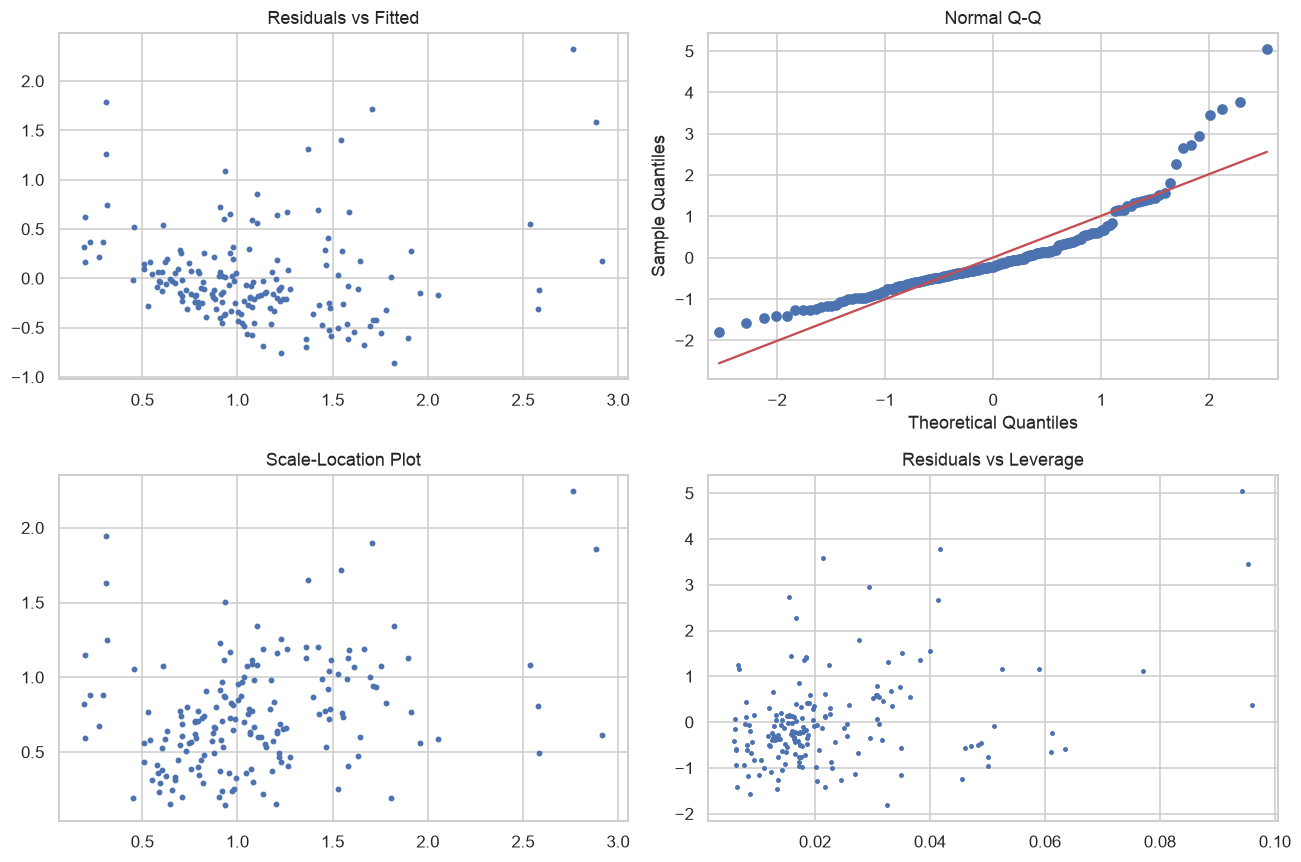
\includegraphics[width=0.75\linewidth]{Residuals vs. fitted values plots.png}
    \caption{\textbf{Residuals vs. Fitted Values Plots}}
    \label{fig:placeholder}
\end{figure}
\vspace{0.8em}
The Ramsey RESET tests whether your model is correctly specified. In Table 7, the p-value is < 0.05, leading us to reject the null hypothesis. This indicates that the linear model likely has misspecification. Therefore, we now consider two new specifications of Model 2: a quadratic model with GDP Growth$^2$ and a model with an interaction between GDP and CCI, as shown below.
\begin{equation}
\text{Volatility}_t = \beta_0 + \beta_1 \,\text{CPI}_t + \beta_2 \,\text{CCI}_t + \beta_3 \,\text{GDP Growth}_t + \beta_4 \,\text{GDP Growth}_t^2 + \varepsilon_t
\label{eq:quadratic}
\end{equation}
\begin{equation}
\text{Volatility}_t = \beta_0 + \beta_1 \,\text{CPI}_t + \beta_2 \,\text{GDP Growth}_t + \beta_3 \,\text{CCI}_t + \beta_4 \,(\text{CPI}_t \times \text{GDP Growth}_t) + \varepsilon_t
\label{eq:interaction}
\end{equation}
\vspace{0.8em}

\begin{table}[H]
\centering
\caption{\textbf{Ramsey RESET Test}}
\label{tab:reset}
\renewcommand{\arraystretch}{1.4}
\begin{tabular}{lcccc}
\toprule
Test & F-statistic & p-value & df (num.) & df (denom.) \\
\midrule
Ramsey RESET & 42.42 & $7.80 \times 10^{-10}$ & 1 & 172 \\
\bottomrule
\end{tabular}
\end{table}
\vspace{0.8em}
Although the interaction model improved the overall model fit, with an adjusted $R^2$ of 0.599 and a positive interaction coefficient between GDP growth and CCI (0.1474), the quadratic model, Model 4, performed better overall (Table 8). The quadratic model has a higher adjusted $R^2$, as well as lower AIC and BIC values, suggesting that it provides a better balance between model fit and complexity. Therefore, the inclusion of the squared GDP growth term appears to better capture the nonlinear relationship between GDP growth and stock market volatility than the interaction between GDP growth and CCI.

\vspace{0.8em}
\begin{table}[H]
\centering
\caption{\textbf{Regression Results: Quadratic vs. Interaction Model}}
\label{tab:model_compare_quad_int}
\renewcommand{\arraystretch}{1.3}
\setlength{\tabcolsep}{16pt}
\begin{tabular}{lcc}
\toprule
 & (1) Quadratic & (2) Interaction \\
\midrule
Intercept & 23.6216$^{***}$ & 37.0422$^{***}$ \\
 & (3.683) & (4.111) \\
CPI & -0.0147$^{***}$ & -0.0139$^{***}$ \\
 & (0.002) & (0.002) \\
CCI & -0.1929$^{***}$ & -0.3306$^{***}$ \\
 & (0.034) & (0.039) \\
GDP Growth & -0.6457$^{***}$ & -14.9575$^{***}$ \\
 & (0.061) & (2.291) \\
GDP Growth$^2$ & 0.2080$^{***}$ & -- \\
 & (0.031) & \\
GDP Growth $\times$ CCI & -- & 0.1474$^{***}$ \\
 & & (0.023) \\
\midrule
Observations & 177 & 177 \\
$R^2$ & 0.617 & 0.608 \\
Adjusted $R^2$ & 0.608 & 0.599 \\
$F$-statistic & 69.24 & 66.59 \\
AIC & 209.6 & 213.9 \\
BIC & 225.5 & 229.8 \\
\bottomrule
\end{tabular}

\vspace{0.5em}
\footnotesize Note: The dependent variable is volatility. Standard errors are in parentheses. $^{***}p<0.001$.
\end{table}

\vspace{0.8em}
With the low p-values (Table 9), we reject the null and can infer that there is statistically significant evidence of heteroskedasticity. The variance of errors is not constant. Heteroskedasticity does not bias coefficients, so we can interpret them as is. However, it does bias standard errors, so we cannot be confident in the amount of uncertainty within these estimates. 

\vspace{0.5em}
\begin{table}[H]
\centering
\caption{\textbf{Heteroskedasticity Tests}}
\label{tab:het_tests}
\renewcommand{\arraystretch}{1.3}
\begin{tabular}{lcc}
\toprule
Test & Test Statistic & $p$-value \\
\midrule
Breusch-Pagan & 13.91856 & 0.00756 \\
White & 30.16518 & 0.00446 \\
\bottomrule
\end{tabular}

\vspace{0.8em}
\end{table}

\vspace{0.8em}
\begin{figure}[H]
    \centering
    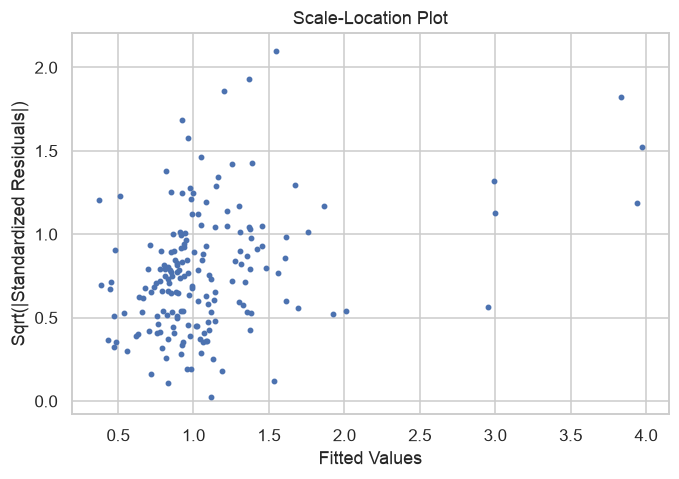
\includegraphics[width=0.5\linewidth]{hetero plot.png}
    \caption{\textbf{Scale-Location Plot}}
    \label{fig:placeholder}
\end{figure}
Most observations are clustered around 0.5-1.5 (Figure 9). This is consistent with the Breusch-Pagan and White test.

\subsection{Outliers and Normality of Residuals}
\begin{figure}[H]
    \centering
    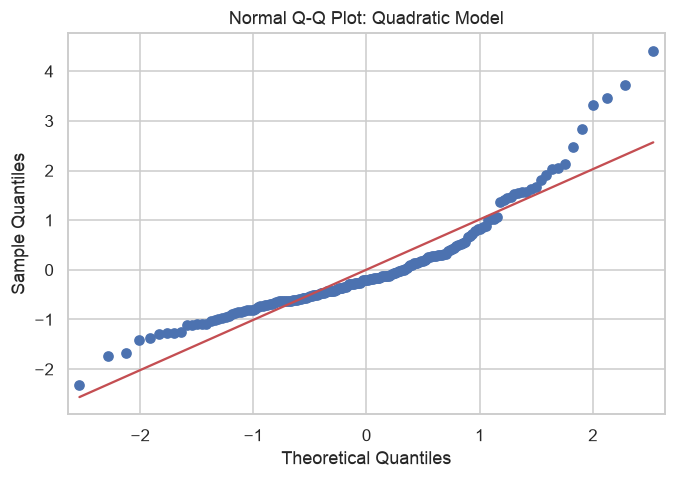
\includegraphics[width=0.5\linewidth]{model2qq.png}
    \caption{\textbf{Quadratic Q-Q Plot}}
    \label{fig:placeholder}
\end{figure}
The Q-Q plot in Figure 10 indicates that our quadratic model does not seem to follow a normal distribution. This is likely due to large outliers and skewness. In Table 10, the $p$-value is far below 0.05, so we reject the null hypothesis of normality.
\begin{figure}
    \centering
    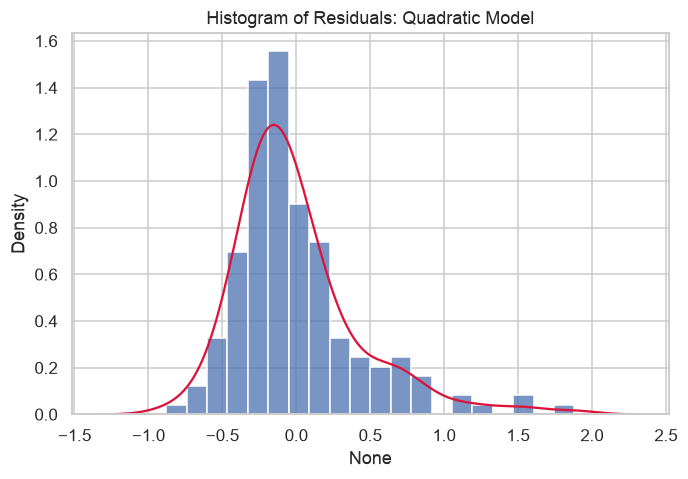
\includegraphics[width=0.5\linewidth]{quad residuals.png}
    \caption{\textbf{Histogram of Quadratic Model's Residuals}}
    \label{fig:placeholder}
\end{figure}
\vspace{0.8em}

\begin{table}[H]
\centering
\caption{\textbf{Jarque-Bera Normality Test}}
\label{tab:jb}
\renewcommand{\arraystretch}{1.3}
\setlength{\tabcolsep}{16pt}
\begin{tabular}{cccc}
\toprule
Jarque-Bera & $p$-value & Skewness & Kurtosis \\
\midrule
145.0 & $3.27 \times 10^{-32}$ & 1.506 & 6.253 \\
\bottomrule
\end{tabular}

\footnotesize Note: The null hypothesis is that the residuals are normally distributed.
\end{table}
\vspace{1em}

\begin{figure}[H]
    \centering
    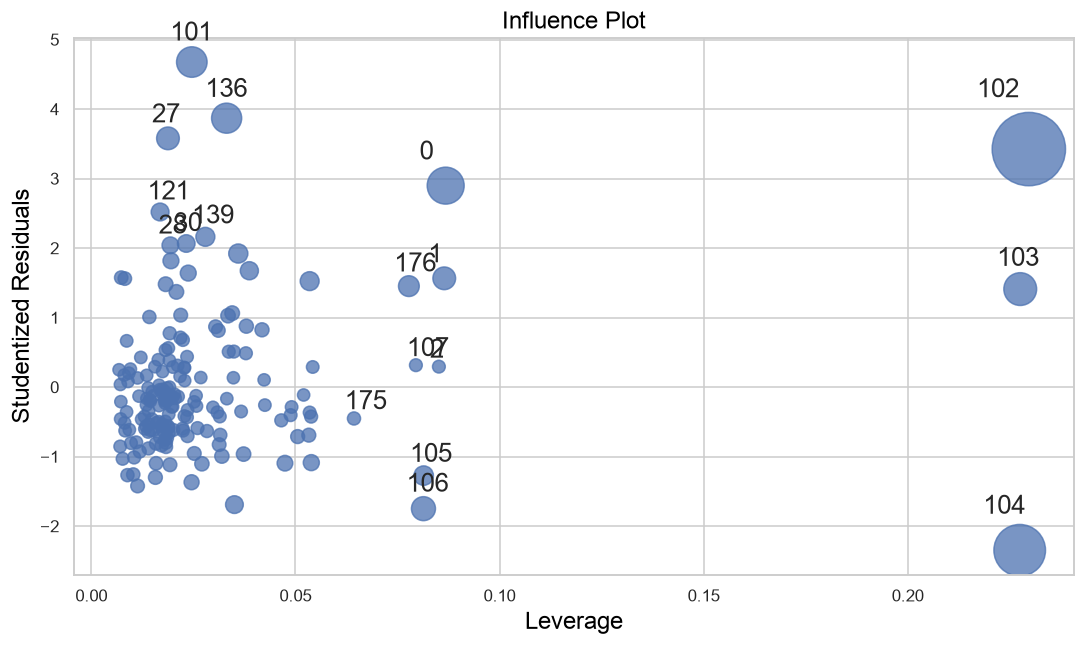
\includegraphics[width=0.5\linewidth]{leverage.png}
    \caption{\textbf{Influence Plot}}
    \label{fig:placeholder}
\end{figure}
\vspace{1em}

\begin{table}[H]
\centering
\caption{\textbf{Influence Diagnostics for the Five Most Influential Observations, sorted to Cooks Distance}}
\label{tab:influence}
\renewcommand{\arraystretch}{1.3}
\setlength{\tabcolsep}{5pt}
\resizebox{\textwidth}{!}{%
\begin{tabular}{rrrrrrrrrrr}
\toprule
Obs. & DFB Int. & DFB GDP & DFB CPI & DFB CCI & DFB GDP$^2$ & Cook's $D$ & Std. Resid. & Leverage & Stud. Resid. & DFFITS \\
\midrule
102 & -0.1537 & -1.5942 & 0.1814 & 0.1541 & 1.4350 & 0.6580 & 3.3220 & 0.2297 & 3.4240 & 1.8695 \\
104 & -0.0118 & 1.0404 & -0.0069 & 0.0068 & -0.9684 & 0.3163 & -2.3179 & 0.2274 & -2.3481 & -1.2740 \\
0 & -0.2117 & -0.1363 & -0.0272 & 0.2294 & 0.6439 & 0.1531 & 2.8376 & 0.0868 & 2.8980 & 0.8934 \\
103 & -0.0046 & -0.6291 & 0.0192 & 0.0067 & 0.5833 & 0.1164 & 1.4056 & 0.2276 & 1.4096 & 0.7651 \\
101 & 0.4492 & 0.0954 & -0.2057 & -0.4555 & -0.2671 & 0.0984 & 4.4161 & 0.0246 & 4.6763 & 0.7428 \\
\bottomrule
\end{tabular}%
}

\vspace{0.5em}
\footnotesize Note: DFB denotes DFBETAS for each coefficient. 
\end{table}
\vspace{0.5em}

Most observations have relatively low leverage in Table 11, but there are a few observations that may be influential (104, 103, 102, 101, etc). These observations may disproportionately affect the estimated regression coefficients. Upon further investigation, we will not be dropping these outliers as 4 out of 5 of them occur during the Great Recession period. In addition, if there are a lot of outliers, chances are, they represent extreme volatility reactions. 

\begin{figure}[H]
    \centering
    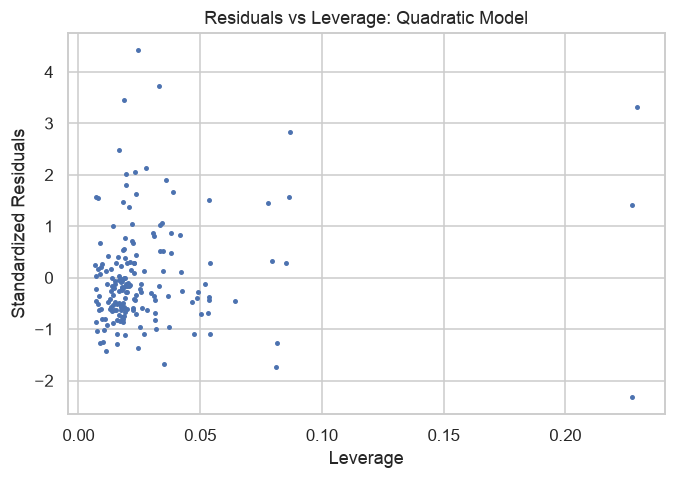
\includegraphics[width=0.5\linewidth]{residuals vs leverage.png}
    \caption{\textbf{Quadratic Model Leverage vs. Residuals}}
    \label{fig:placeholder}
\end{figure}

Most observations have relatively low leverage, as they are clustered between 0.01 and 0.05 (Figure 13). However, some observations have unusually large residuals, exceeding 4 standard deviations. This suggests that actual stock market volatility was considerably higher than what the model predicted for these observations. There are also a few observations on the right side of the plot, near 0.20, which may indicate unusual combinations of macroeconomic predictor values. Overall, the plot suggests that potentially influential observations are present, which could affect the estimated coefficients. This is consistent with the results from Cook's Distance (Table 11).

\vspace{0.8em}
\begin{table}[H]
\centering
\caption{\textbf{Largest Absolute DFBETAS by Coefficient}}
\label{tab:dfbetas_max}
\renewcommand{\arraystretch}{1.3}
\setlength{\tabcolsep}{16pt}
\begin{tabular}{lc}
\toprule
Coefficient & Max $|\text{DFBETAS}|$ \\
\midrule
GDP Growth & 1.594179 \\
GDP Growth$^2$ & 1.434972 \\
CCI & 0.535871 \\
Intercept & 0.516201 \\
CPI & 0.357364 \\
\bottomrule
\end{tabular}
\end{table}
\vspace{0.8em}

DFBETAS measure how much each regression coefficient changes, in standard errors, when a single observation is removed. At least one observation substantially influences the estimated GDP growth coefficient, while another influential observation affects the estimated nonlinear relationship between GDP growth and volatility (Table 12, depicted by DFBETA > 1).

\subsection{Model Validation and Robustness}
\begin{figure}[H]
    \centering
    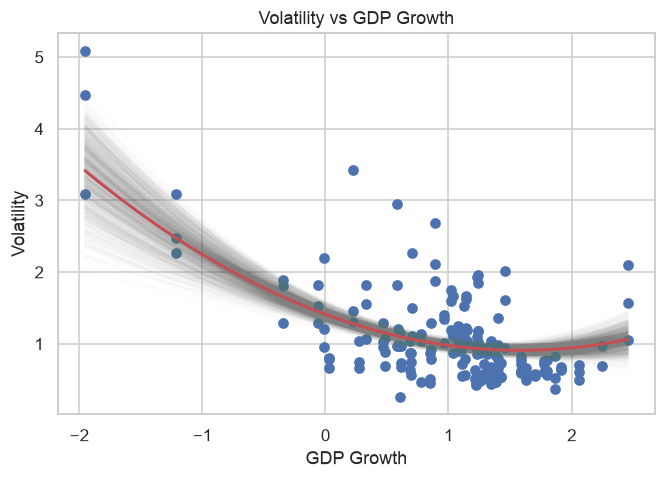
\includegraphics[width=0.5\linewidth]{bootstrapping.png}
    \caption{\textbf{Bootstrap Coefficient Estimates}}
    \label{fig:placeholder}
\end{figure}
\vspace{0.8em}

Figure 14 illustrates a nonlinear, U-shaped relationship between GDP growth and stock market volatility. The blue points represent observed volatility values, while the gray curves represent 1,000 bootstrap samples, with the red line showing the average relationship across the bootstrap estimates. Volatility generally decreases as GDP growth increases, before the estimated relationship begins to turn slightly upward at higher GDP growth rates.
\vspace{0.8em}

\begin{figure}[H]
    \centering
    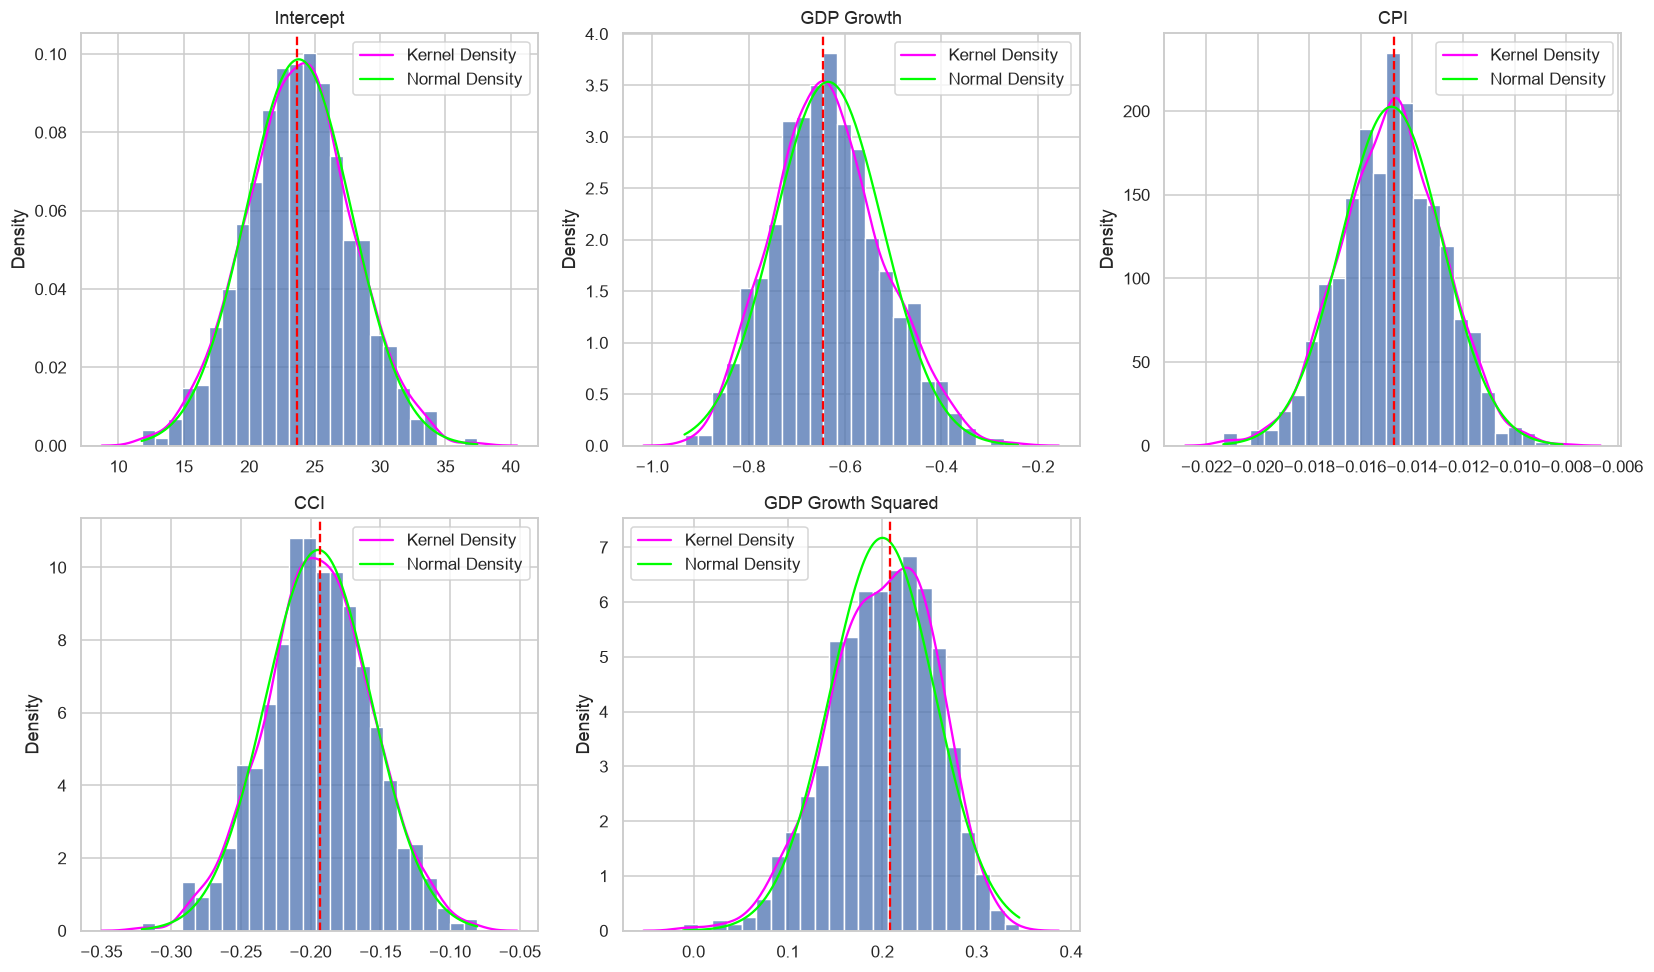
\includegraphics[width=0.75\linewidth]{estimate comparison.png}
    \caption{\textbf{Bootstrap Sample Distribution}}
    \label{fig:placeholder}
\end{figure}

\begin{figure}[H]
    \centering
    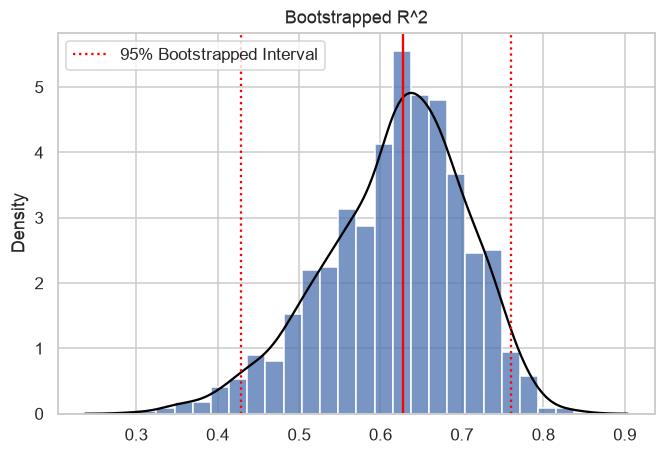
\includegraphics[width=0.5\linewidth]{bootstrap comparison.png}
    \caption{\textbf{Bootstrap $R^2$}}
    \label{fig:placeholder}
\end{figure}

The bootstrap distributions (Figure 15) appear relatively bell-shaped, with GDP growth exhibiting some symmetry. The bootstrap estimates are also close to the original OLS estimates (Table 13), suggesting that the results are relatively consistent across samples. Additionally, the mean of the coefficient for GDP growth squared remains positive, supporting the nonlinear, U-shaped relationship between GDP growth and volatility.

\vspace{0.8em}
\begin{table}[H]
\centering
\caption{\textbf{OLS vs. Bootstrap Coefficient Estimates}}
\label{tab:bootstrap}
\renewcommand{\arraystretch}{1.3}
\setlength{\tabcolsep}{8pt}
\begin{tabular}{lccccc}
\toprule
Variable & OLS Estimate & Bootstrap Mean & Bootstrap Std. Error & 2.5th Percentile & 97.5th Percentile \\
\midrule
Intercept & 23.6216 & 23.7898 & 4.0457 & 15.7867 & 31.8590 \\
CPI & -0.0147 & -0.0148 & 0.0020 & -0.0187 & -0.0110 \\
CCI & -0.1929 & -0.1944 & 0.0381 & -0.2710 & -0.1193 \\
GDP Growth & -0.6457 & -0.6348 & 0.1130 & -0.8350 & -0.4034 \\
GDP Growth$^2$ & 0.2080 & 0.2002 & 0.0556 & 0.0867 & 0.2983 \\
\bottomrule
\end{tabular}
\end{table}
\vspace{0.8em}

We conducted a 5-fold cross-validation test using the quadratic volatility model, which produced a mean RMSE of 0.5268 (Table 14). The values ranged from 0.3417 to 0.7215 across the five folds. This suggests that the model's predictive accuracy varies across different samples, meaning its performance may differ depending on the time period being evaluated. The quadratic model has an average out-of-sample prediction error (RMSE) of approximately 0.527 percentage points of daily-return volatility.

\vspace{0.8em}
\begin{table}[H]
\centering
\caption{\textbf{5-Fold Cross-Validation RMSE}}
\label{tab:cv_rmse}
\renewcommand{\arraystretch}{1.3}
\setlength{\tabcolsep}{10pt}
\begin{tabular}{lcccccc}
\toprule
 & Fold 1 & Fold 2 & Fold 3 & Fold 4 & Fold 5 & Mean \\
\midrule
RMSE & 0.7215 & 0.5054 & 0.5542 & 0.5112 & 0.3417 & 0.5268 \\
\bottomrule
\end{tabular}
\end{table}
\vspace{0.8em}
The OLS assumption tests revealed several potential violations that should be considered when interpreting the model's results. First, both the Breusch-Pagan test (p = 0.00756) and White test (p = 0.00446) produced p-values below 0.05, leading us to reject the null hypothesis of constant variance. This indicates the presence of heteroskedasticity, meaning the variance of the residuals changes across observations. Although this does not bias the OLS coefficient estimates, it can make conventional standard errors and confidence intervals unreliable, affecting our statistical inference. Additionally, the Jarque-Bera test (JB = 145, p < 0.001) led us to reject the assumption of normally distributed residuals. The residual distribution also showed positive skewness and excess kurtosis, suggesting the presence of extreme observations that may affect the reliability of our inference. In terms of model specification, the original OLS model failed the Ramsey RESET test, suggesting potential misspecification. However, including the square of GDP growth improved the model fit, as reflected by the adjusted $R^2$, AIC, and BIC values. Finally, we conduct a robustness analysis using 1,000 bootstrap replications. This produced coefficient means similar to the original OLS estimates, providing some stability in the estimated relationships. The 5-fold cross-validation test produced a mean RMSE of 0.5268, indicating that predictive accuracy varies across different samples and time periods. Overall, while the quadratic model improves upon the original specification, the violations of the OLS assumptions mean that the results, particularly the statistical inference, should be interpreted with some caution.

\section{Results and Economic Interpretation}
\begin{table}[H]
\centering
\caption{\textbf{OLS Regression Results: Model with Squared GDP Growth}}
\label{tab:ols_quadratic}
\renewcommand{\arraystretch}{1.3}
\begin{tabularx}{\textwidth}{Xrrrrrr}
\toprule
Variable & Coefficient & Std. Error & $t$-statistic & $p$-value & 95\% CI Lower & 95\% CI Upper \\
\midrule
Intercept & 23.6216 & 3.683 & 6.414 & $<0.001$ & 16.352 & 30.891 \\
CPI & -0.0147 & 0.002 & -6.692 & $<0.001$ & -0.019 & -0.010 \\
CCI & -0.1929 & 0.034 & -5.664 & $<0.001$ & -0.260 & -0.126 \\
GDP Growth & -0.6457 & 0.061 & -10.581 & $<0.001$ & -0.766 & -0.525 \\
GDP Growth$^2$ & 0.2080 & 0.031 & 6.734 & $<0.001$ & 0.147 & 0.269 \\
\midrule
Observations & \multicolumn{6}{r}{177} \\
$R^2$ & \multicolumn{6}{r}{0.617} \\
Adjusted $R^2$ & \multicolumn{6}{r}{0.608} \\
$F$-statistic & \multicolumn{6}{r}{69.24}\\
AIC & \multicolumn{6}{r}{209.6} \\
BIC & \multicolumn{6}{r}{225.5} \\
\bottomrule
\end{tabularx}
\vspace{0.8em}

\footnotesize Note: The dependent variable is volatility.
\end{table}
When CPI increases by one point, we expect the monthly standard deviation of daily percentage returns (volatility) to decrease by approximately 0.015 percentage-points on average, holding CCI and GDP growth constant (Table 15). CCI has a similar effect. When CCI increases by one point, we can expect volatility to decrease by approximately 0.193 percentage-points on average, holding CPI and GDP constant. Our two GDP coefficients must be interpreted together, as it is impossible to increase one and not the other. Therefore, we interpret its marginal effect (derivative). 
\begin{equation*}
\begin{split}
\frac{\partial\, \text{Volatility}}{\partial\, \text{GDP Growth}} &= -0.646 + 2(0.208)\,\text{GDP growth} \\
&= -0.646 + 0.416\,\text{GDP Growth}
\end{split}
\label{eq:marginal_gdp}
\end{equation*}
Volatility begins to increase when GDP growth is greater than approximately 1.553\% (0.646/0.416 = 1.553). All coefficients in our final model have 95\% confidence intervals that exclude zero, meaning that each predictor is statistically significant at the 5\% level. While our coefficients are relatively small, we must determine economic significance in terms of volatility. Changes in volatility may have different implications for investors depending on the size of their investments, and overall exposure to the stock market. Therefore, the economic significance of this relationship may vary greatly by individual. \\
\indent The adjusted $R^2$ determines how well our model predicts the variation in volatility, while accounting for the loss of degrees of freedom in adding predictors. An $R^2$ of 0.608 is relatively high, meaning that approximately 61\% of the variation in volatility is explained by our model. 

\section{Limitations, Policy Implications, and Extensions}
\subsection{Key Limitations and Bias}
Throughout our analysis, we encountered several limitations that should be considered when interpreting our results. The variables of GDP growth and CPI exhibited an extremely high correlation of 0.99 (pre-GDP transformation), when we generated the correlation heatmap. Since both variables generally trend upward over time, including them together in their original forms could make it difficult to isolate their individual relationships with stock market volatility. To address this concern, we transformed GDP and measured the monthly growth rates rather than using its original quarterly levels. Secondly, our sample size decreased after merging our various datasets. Although our original S\&P 500 dataset contained 3,773 daily observations, we had to calculate volatility on a monthly basis to match the frequency of our macroeconomic variables. This reduced our dataset to 180 total observations, and after accounting for the first 3 missing GDP growth values, our final regression includes 177 observations. The need to maintain consistency across our variables resulted in a smaller sample size, which limited the amount of information available for our regression analysis and may have reduced the precision of our estimates.\\
\indent The variables of Fed. Reserve IR Change and Un. Rate Change were not identified as statistically significant. This limited our ability to draw meaningful conclusions about their relationship with volatility. Another transformation was applied, calculating the percentage point difference between the previous month and current month. After re-running our regression tests, both variables came out as statistically significant. \\
\indent Our regression diagnostics identified several violations of OLS assumptions. The Breusch-Pagan and White tests indicated the presence of heteroskedasticity, while the Jarque-Bera test showed that our residuals were not normally distributed. These issues may affect the reliability of our standard errors, confidence intervals, and statistical significance. Another limitation we encountered was the presence of influential observations in our dataset. Through Cook’s distance and influence plots, we identified several observations that had a relatively large influence on our regression estimates, particularly during the Great Recession. These observations may have affected our estimated coefficients and contributed to some of the issues identified in our regression diagnostics, including non-normality and heteroskedasticity. However, we also had to consider whether removing these observations was appropriate given our research question. Since our analysis specifically focuses on stock market volatility surrounding the Great Recession, removing these observations could exclude some of the most important periods of financial instability. Therefore, we decided to retain them while acknowledging that their influence may affect the reliability of our estimates. \\
\indent One potential source of bias in our analysis is omitted variable bias (OVB). Although we included several macroeconomic indicators, there are many other factors that could influence stock market volatility that were not accounted for in our regression. For example, investor expectations, financial market uncertainty, and international economic events could all affect volatility. If these omitted factors are correlated with our explanatory variables, our estimated coefficients may be biased, making it difficult to isolate the individual relationship between each variable and volatility. Reverse causality is also a concern. For example, while changes in consumer confidence may influence stock market volatility, increased volatility could also affect how confident consumers feel about the economy. Similarly, changes in the federal reserve interest rate may be a response to economic instability rather than an independent cause of volatility. As a result, we cannot necessarily interpret our estimated coefficients as causal effects. 
\subsection{Policy Implications, Research Extensions, and External Validity}
Our findings suggest that broader macroeconomic conditions, particularly GDP growth, CPI, and CCI, are significantly associated with stock market volatility. These relationships may provide useful insights for policymakers when evaluating economic conditions and identifying periods of increased financial instability. In particular, understanding the relationship between economic growth, consumer confidence, and stock market volatility may help policymakers monitor changes in financial market conditions, especially during periods of economic downturn. Additionally, our findings emphasize the importance of considering multiple economic indicators rather than relying on a single measure when assessing overall financial stability. \\
\indent Future research could build upon our analysis by exploring alternative estimation methods and incorporating additional explanatory variables. To address the heteroskedasticity identified in our regression diagnostics, future research could consider using Generalized Least Squares (GLS) or Weighted Least Squares (WLS). These methods could account for differences in error variance across observations, potentially improving the efficiency of the estimates and the reliability of statistical inference. Additionally, future research could address potential omitted variable bias by incorporating other financial market indicators, such as the VIX or Treasury yields. Including these variables could capture additional factors influencing stock market volatility and potentially improve the explanatory power of the model. \\
\indent The findings of our analysis are primarily applicable to the U.S. stock market between 2000 and 2014, with particular emphasis on the period surrounding the Great Recession. Although our original datasets covered a broader time frame, we restricted our analysis to this period to examine how stock market volatility behaved before, during, and after the recession. As our analysis uses the S\&P 500 stock market, which primarily represents large publicly traded U.S. companies, our findings may not be generalizable to smaller companies, international stock markets, or other types of financial assets. The Great Recession was largely driven by the collapse of the U.S. housing market and the subsequent financial crisis. However, other economic downturns may differ in their underlying causes and consequences. Therefore, the relationships observed between macroeconomic conditions and stock market volatility may not necessarily hold during other recessions or periods of economic instability.


\clearpage
\nocite{*}
\bibliographystyle{plainnat}
\bibliography{main}

\section{Appendix}
\subsection{Box Plots of Remaining Continuous Variables}
\begin{figure}[H]
    \centering
    \begin{subfigure}[b]{0.48\textwidth}
        \centering
        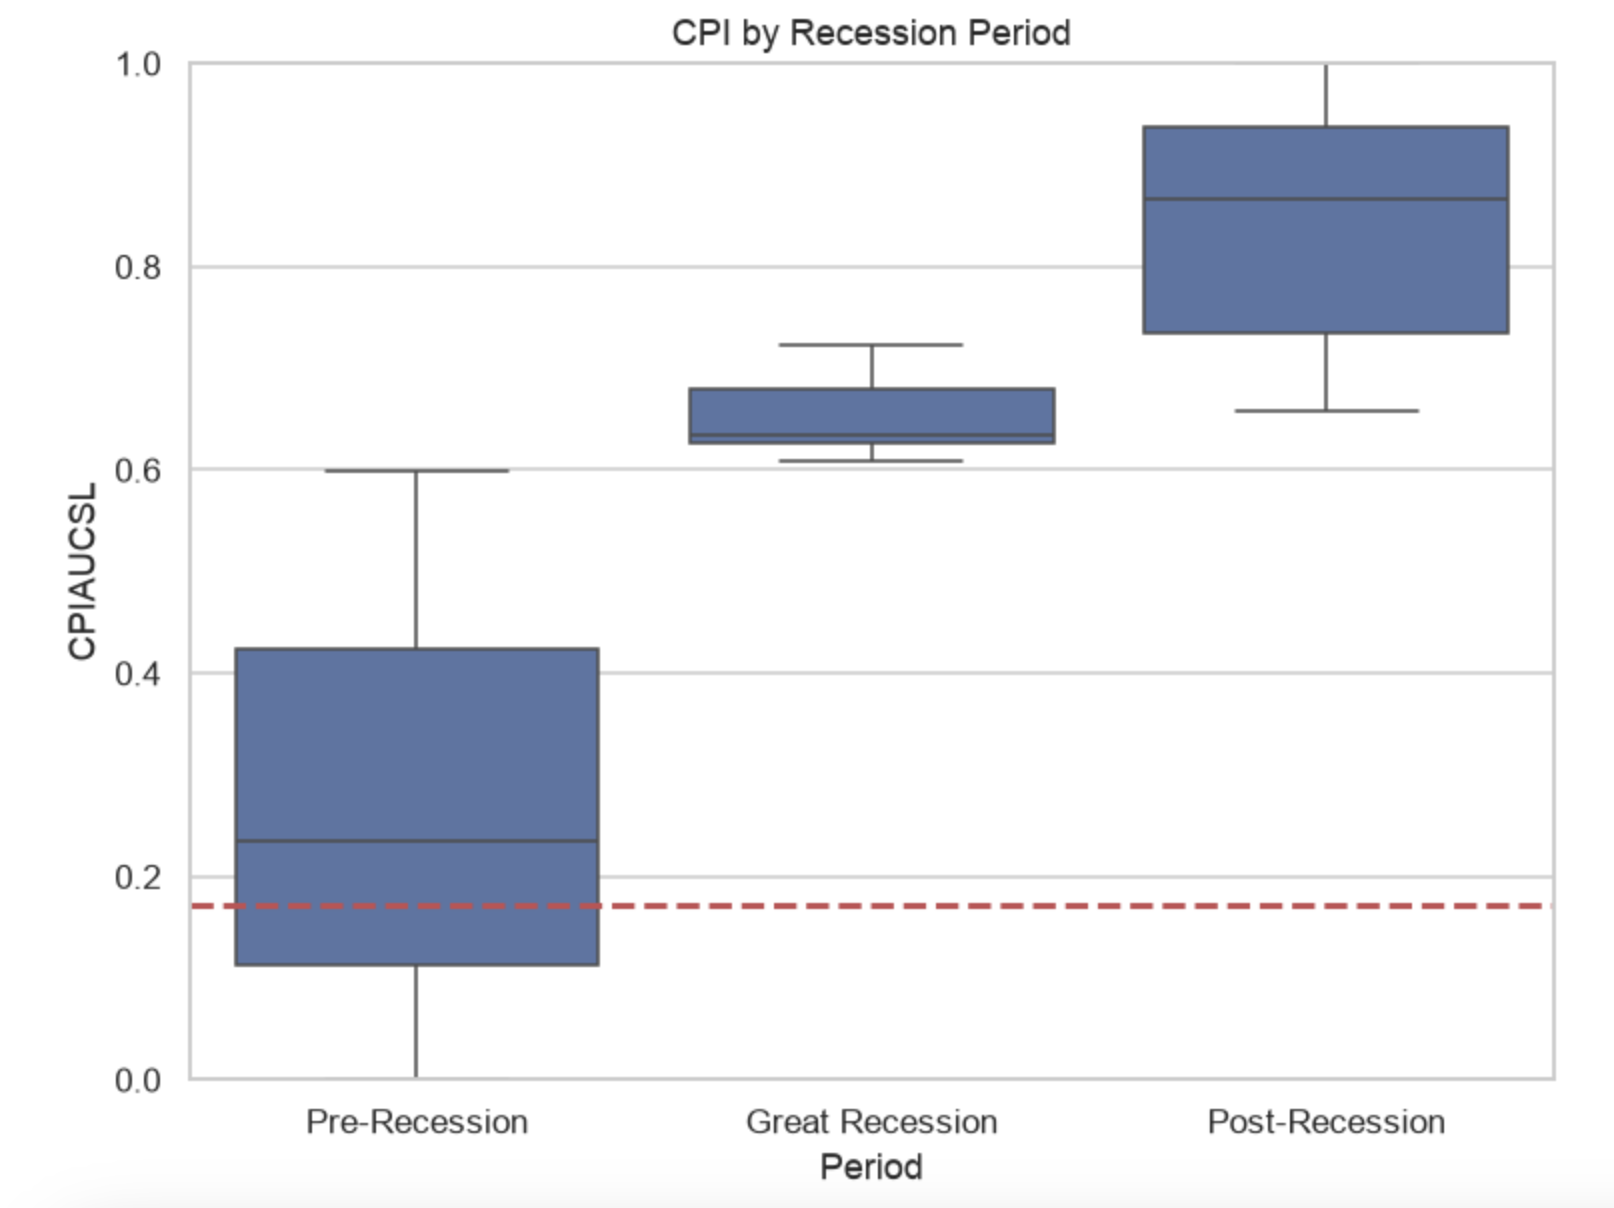
\includegraphics[width=\linewidth]{CPI boxplot.png}
        \caption{\textbf{CPI Box Plot}}
        \label{fig:cpi_box}
    \end{subfigure}
    \hfill
    \begin{subfigure}[b]{0.48\textwidth}
        \centering
        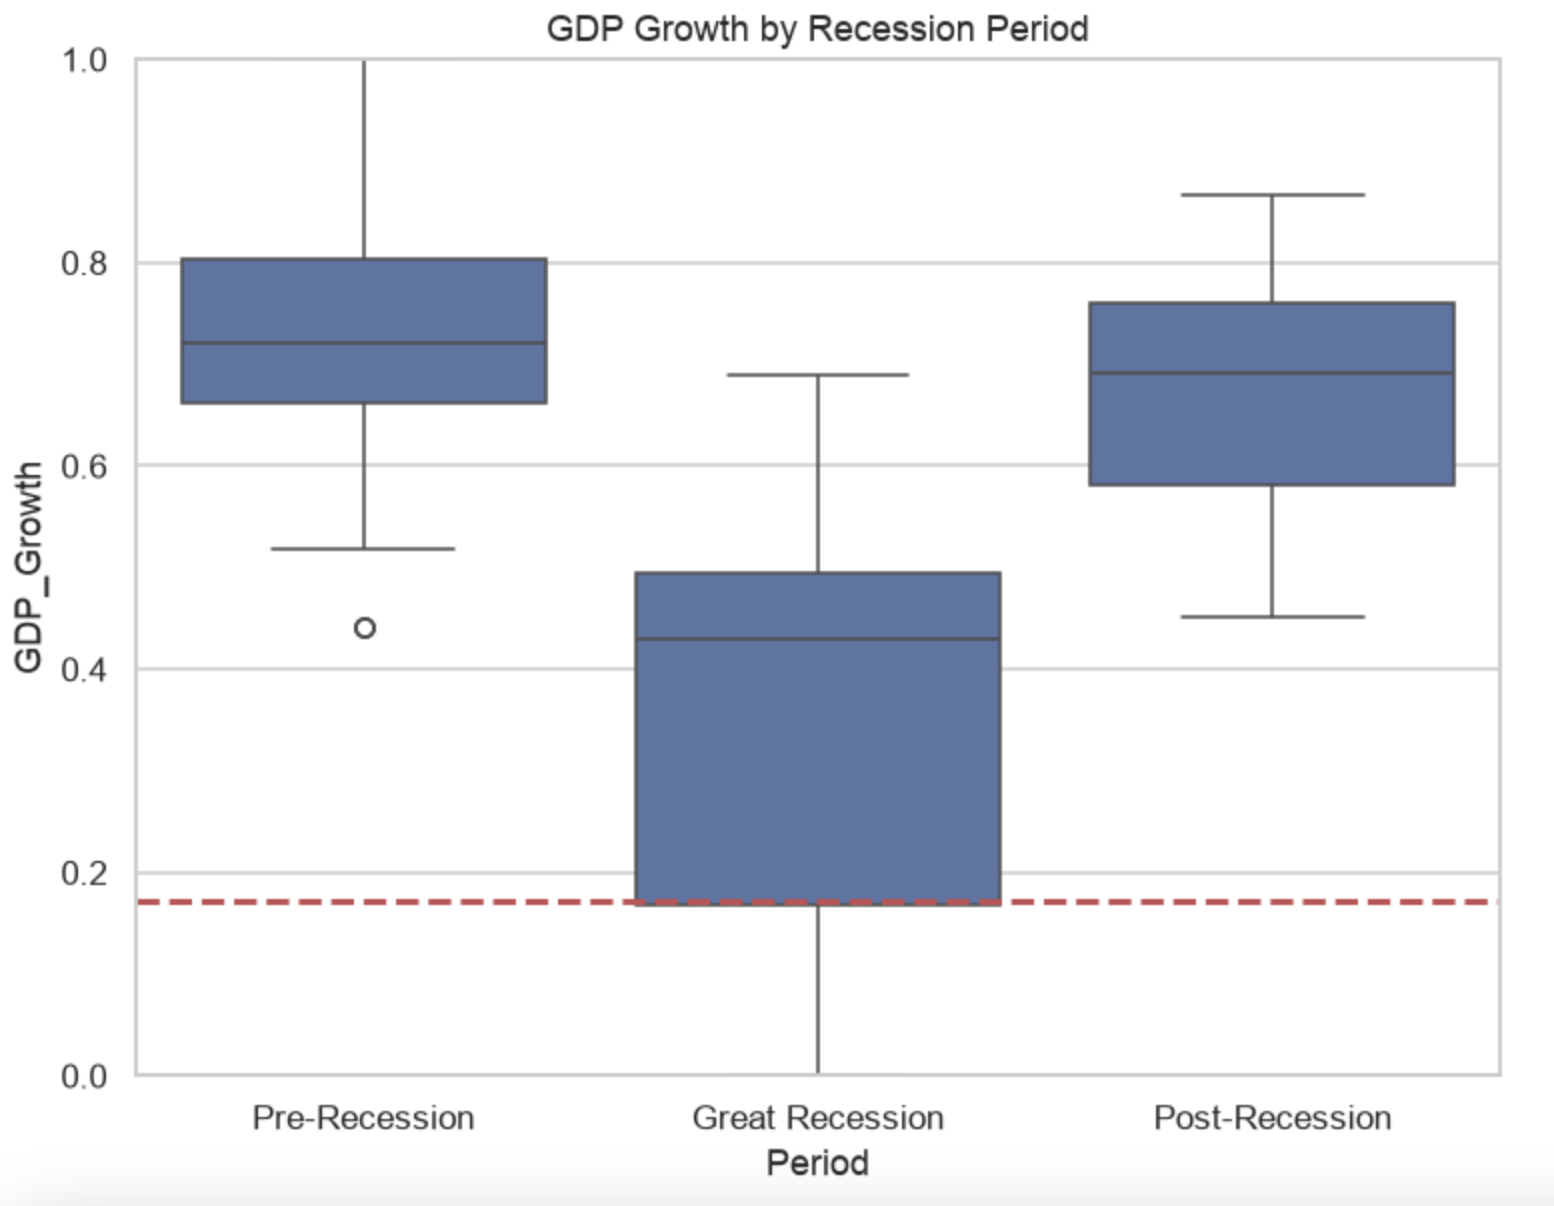
\includegraphics[width=\linewidth]{GDP boxplot.png}
        \caption{\textbf{GDP Growth Box Plot}}
        \label{fig:gdp_box}
    \end{subfigure}

    \vspace{1em}

    \begin{subfigure}[b]{0.48\textwidth}
        \centering
        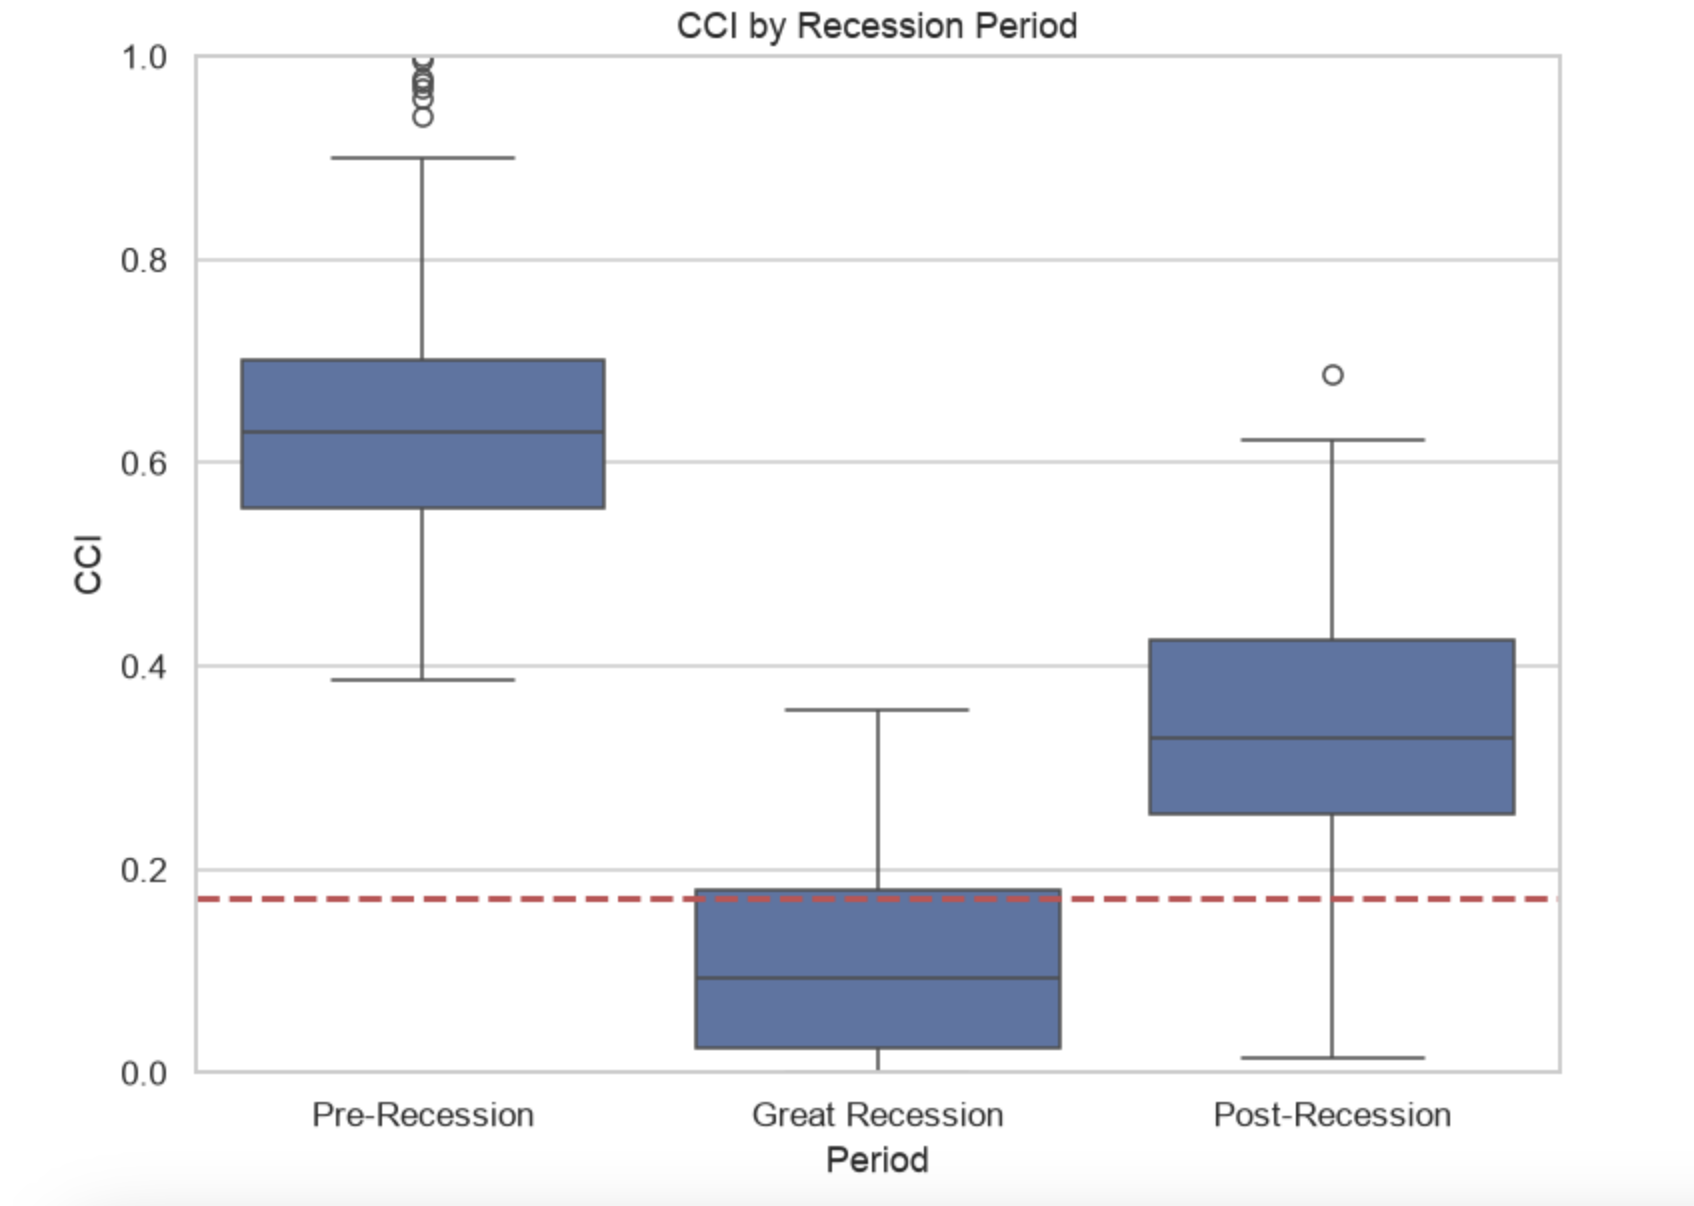
\includegraphics[width=\linewidth]{CCI Box Plot.png}
        \caption{\textbf{CCI Box Plot}}
        \label{fig:cci_box}
    \end{subfigure}

    \caption{\textbf{Box Plots by Recession Period}}
    \label{fig:boxplots}
\end{figure}
\vspace{0.8em}

\subsection{Q-Q Plots of Remaining Variables}
\begin{figure}[H]
    \centering
    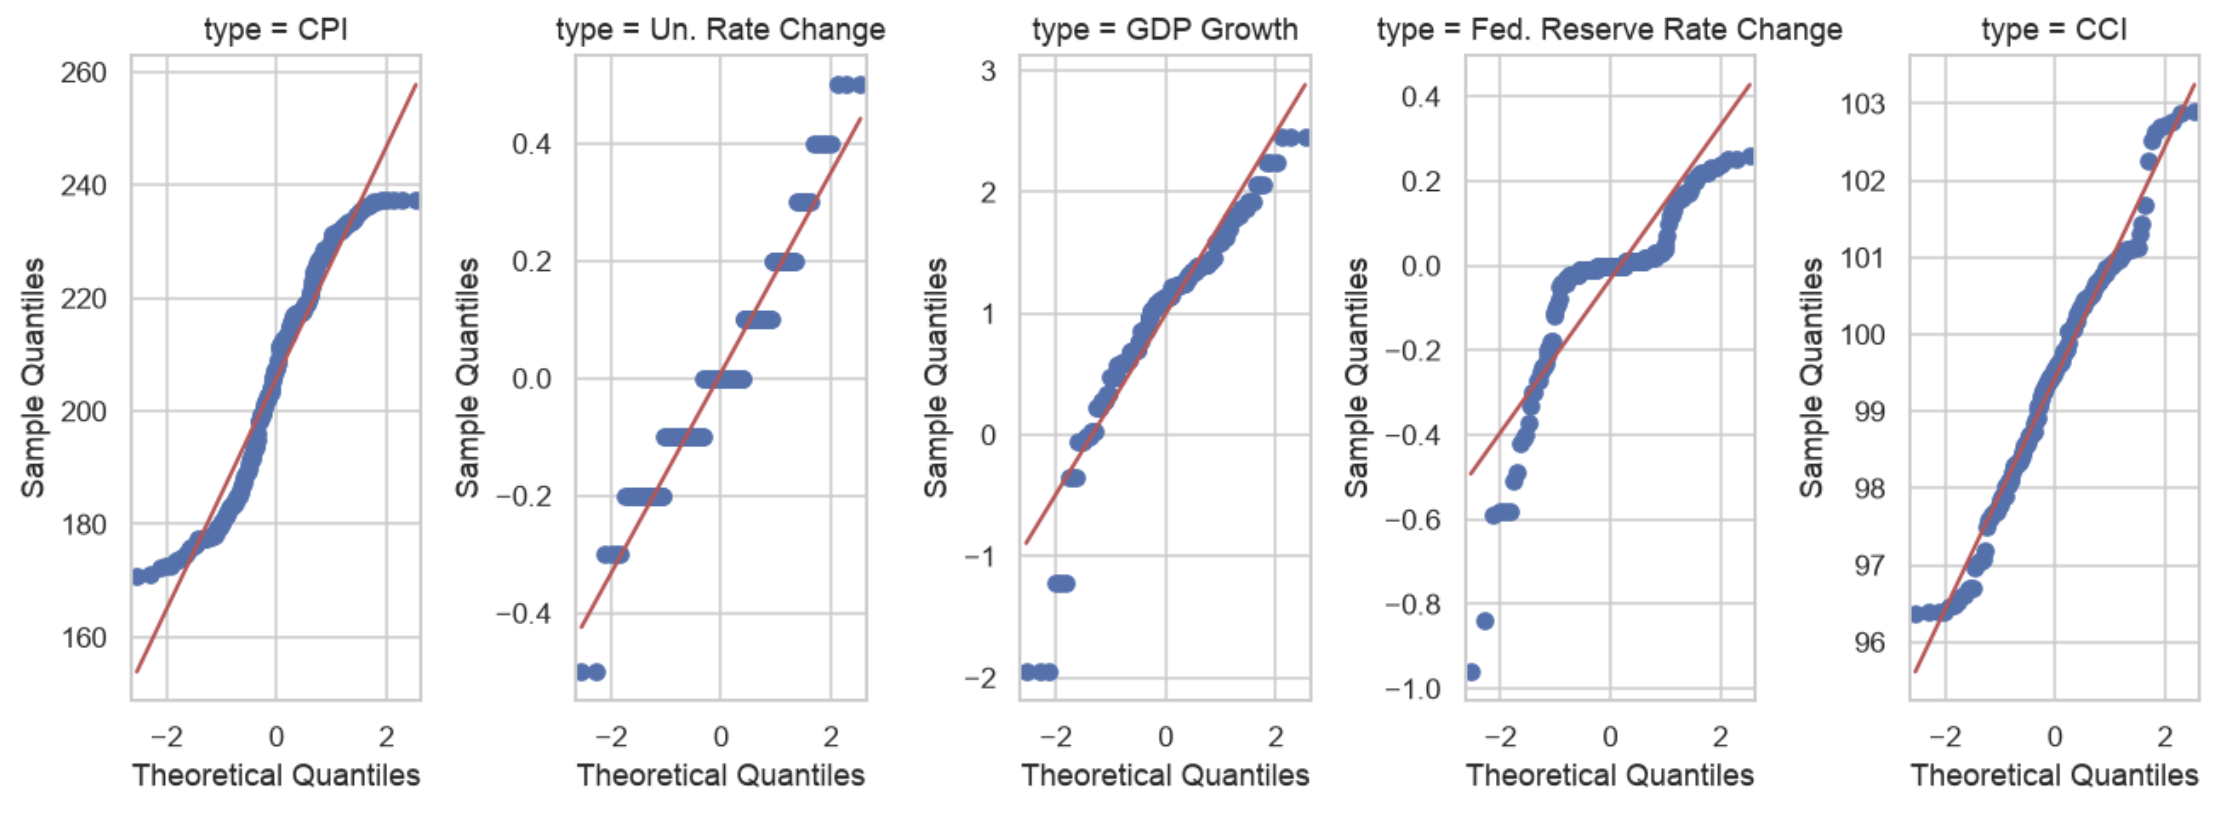
\includegraphics[width=0.75\linewidth]{Remaining QQ plots.png}
    \caption{\textbf{Q-Q Plots}}
    \label{fig:placeholder}
\end{figure}
\vspace{0.8em}
\begin{figure}[H]
    \centering
    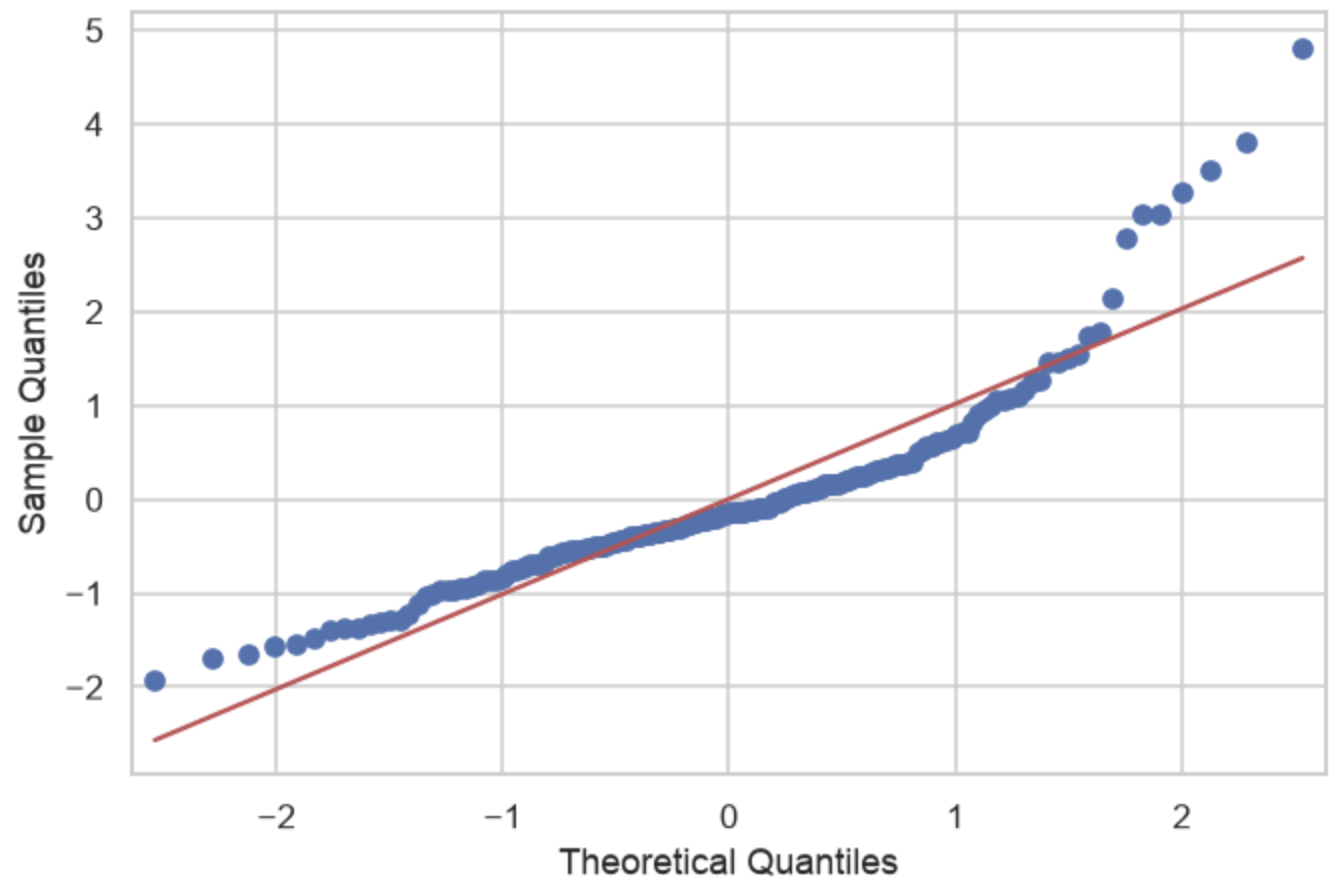
\includegraphics[width=0.5\linewidth]{QQ of standardized resid.png}
     \caption{\textbf{Q-Q Plot of Standardized Residuals}}
    \label{fig:placeholder}
\end{figure}
Figure 18 above shows the Q-Q plots of remaining predictors. The plots of Un. Rate Change and the Fed. Reserve IR Change cannot be interpreted as they are not continuous variables. All other Q-Q plots demonstrate normality, though with varying degrees. The Q-Q plot of residuals in Figure 19 show some residuals deviating from the normal distribution, at the ends. This is similar to that of the Q-Q plot of Volatility (Figure 5).

\subsection{Density Plots of Remaining Variables}
\begin{figure}[H]
    \centering
    \begin{subfigure}[b]{0.48\textwidth}
        \centering
        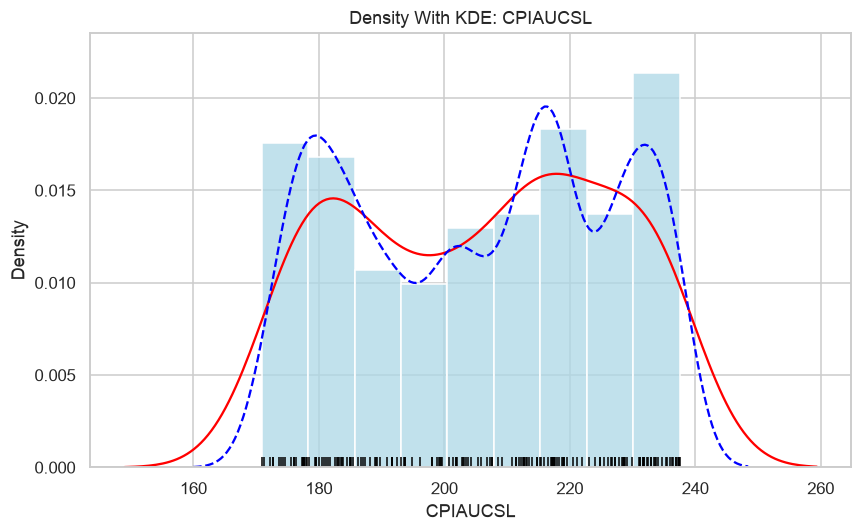
\includegraphics[width=\linewidth]{CPI density.png}
        \caption{\textbf{CPI Density}}
        \label{fig:cpi_density}
    \end{subfigure}
    \hfill
    \begin{subfigure}[b]{0.48\textwidth}
        \centering
        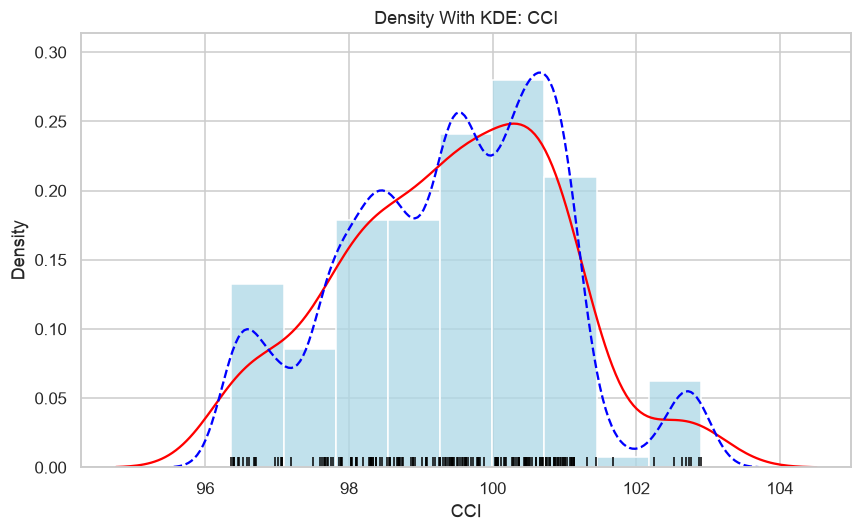
\includegraphics[width=\linewidth]{CCI Density.png}
        \caption{\textbf{CCI Density}}
        \label{fig:cci_density}
    \end{subfigure}

    \vspace{1em}

    \begin{subfigure}[b]{0.48\textwidth}
        \centering
        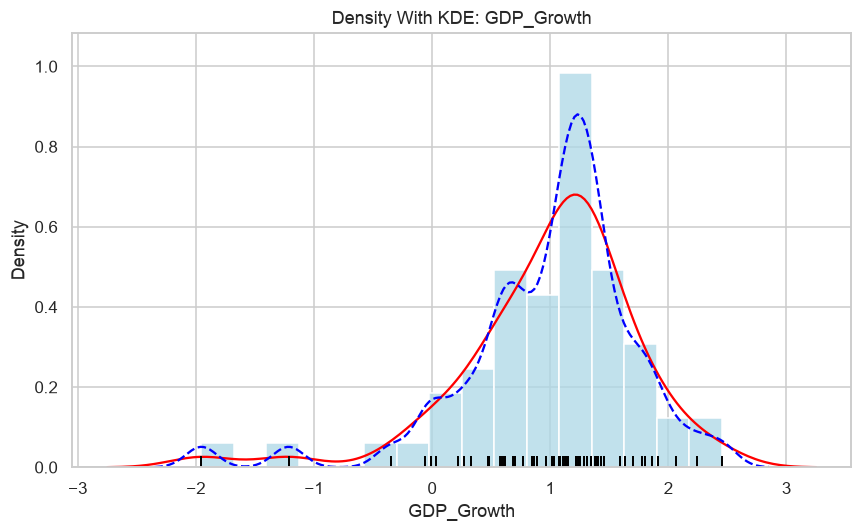
\includegraphics[width=\linewidth]{GDP Density.png}
        \caption{\textbf{GDP Growth Density}}
        \label{fig:gdp_density}
    \end{subfigure}

    \caption{\textbf{Density Plots of the Model Variables}}
    \label{fig:densities}
\end{figure}
%\input project components?
\end{document}